\documentclass[10pt, a4paper]{article}

% Fundamentals & Fonts
\usepackage[utf8]{inputenc}
\usepackage[T1]{fontenc}
\usepackage{lmodern}
\usepackage{microtype}
\usepackage{geometry}
\newgeometry{textwidth = 16cm, textheight=25cm}

% Math & Logic
\usepackage{amsmath, amssymb}
\usepackage{amsthm} 
\usepackage{enumitem}
% Define the "Assumption" environment
\theoremstyle{assumption}
\newtheorem{assumption}{Assumption}[section]
\newtheorem{example}{Example}[section]
\newtheorem{remark}{Remark}[section]
\theoremstyle{definition}
\newtheorem{definition}{Definition}[section]
\theoremstyle{theorem}
\newtheorem{theorem}{Theorem}[section]
% Graphics & TikZ
\usepackage{graphicx}
\usepackage{subcaption}
\usepackage{svg}
\usepackage{tikz}
\usepackage{pdfpages}
\usepackage{wrapfig}

% Professional Tables (Crucial for SI)
\usepackage{booktabs}
\usepackage{longtable}
\usepackage{array}
\usepackage{multirow}
\usepackage{adjustbox}
\usepackage{threeparttable} % From SI
\usepackage{siunitx}        % From SI (For Table S7)
\usepackage{lscape}

% Layout & Formatting
\usepackage{float}
\usepackage{xcolor}
\usepackage{soul}
\usepackage{caption}
\usepackage{authblk}
\usepackage{layout}
% Bibliography & Citations
\usepackage{natbib}

\usepackage{mdframed}
% Define a custom environment
\newmdenv[
  backgroundcolor=gray!20,   % background shade
  linecolor=black,           % border color
  roundcorner=5pt,           % rounded corners (optional)
  linewidth=0pt,             % border thickness
  innertopmargin=0pt,      % reduce top spacing
  innerbottommargin=5pt
]{shaded}

% Links
\usepackage[hidelinks]{hyperref}
% \hypersetup{
%     colorlinks=true,
%     linkcolor=blue,
%     citecolor=blue,
%     urlcolor=cyan
% }

% --- MACROS ---
\newcommand{\R}{\mathbb{R}}
\newcommand{\E}{\mathbb{E}}
\newcommand{\V}{\mathrm{Var}}
\newcommand{\Cov}{\mathrm{Cov}}


\newtheorem{lemma}{Lemma}
\newtheorem{proposition}{Proposition}


\title{\textbf{Title}}
\author[]{}
% \author[1]{Antonio Panico\thanks{Email: antonio.panico@unipr.it}}
%\author[2]{Andrew Burlinson}
%\author[1]{Luigi Grossi}

% \affil[1]{Department of Engineering for Industrial Systems and Technologies, University of Parma, 43124 Parma, Italy}
%\affil[2]{School of Economics, University of Sheffield, Sheffield, UK}
%\email{Antonio.panico@unipr.it}

\date{} % <-- niente data

\begin{document}

\maketitle

\begin{abstract}
    We developed a unified non-parametric framework for change-point detection in multivariate, locally 
stationary time series defined via nonlinear moment equations $\mathbb{E}[H(X_{t,n}, \theta_{t,n})] = 0$. The proposed 
methodology encompasses a broad range of statistical targets, including robust location, time-varying $M$-
regression with redescending score functions, autocovariances, and smoothed extremal downside 
correlation (SEDC) densities. To circumvent the slow convergence rates and boundary bias inherent to 
standard plug-in estimators, we construct a linearized partial-sum estimator based on a local one-step Taylor 
expansion with an independent decoupling lag. Under mild physical dependence conditions and smooth 
kernel assumptions, we establish uniform consistency of the local pilot estimators and prove a Functional 
Central Limit Theorem (FCLT) in the Skorokhod space, showing weak convergence of the linearized process 
toward a Gaussian martingale driven by the local long-run covariance structure. Furthermore, we prove the 
validity of a multiplier block bootstrap to approximate the asymptotic null distribution of the resulting 
CUSUM test statistic. Extensive Monte Carlo simulations demonstrate that the proposed linearized CUSUM 
test maintains accurate nominal size under severe nuisance non-stationarity and heavy-tailed innovations, 
while achieving substantial power gains and bias reduction over classical baselines under additive, 
innovation, and replacement outlier regimes.

\end{abstract}

\section{Introduction}
% In recent years, the European electricity market has faced several challenges,
% particularly due to external shocks and evolving policy goals. Indeed, the wholesale electricity market has been characterized by extreme volatility during the period from 2020 to 2025, caused by both geopolitical events,
% most notably the Ukraine-Russia war and the resulting gas price crisis, and market-specific factors such as the COVID-19 pandemic.
% Previous research has focused on measuring extremal dependence \cite{Lindstrom2012} and utilizing network frameworks to analyze volatility spillovers and profitability linkages among energy markets \cite{Felix2025}.
% This study aims to provide a more comprehensive characterization of time-varying extremal dependence by developing a CUSUM test statistic for changes in Extreme Dependences.
% Interesting, our framework aligns with the literature of changes in extreme dependence, which is relevant for many applications, i.e., environments,  earth sciences, and finance. 

% An effective approach to monitoring the evolution of extremal dependence is the application of continuous time-varying models. Within this framework, \cite{Castro2018, Hoga2022, Gong2022} developed semi-parametric regression models to dynamically track these shifts. However, these models do not offer formal statistical tests to detect structural change points in extremal dependence.

% Historically, structural break testing in financial and extreme value contexts has focused on other characteristics. For instance, the seminal work of \cite{Longin2001} derived a formal statistical method to test for changes in conditional correlations , likewise \cite{Barassi2020} developed a semiparametric test based on CUSUM to detect changes in correlation structure conditioning on time. In extreme value theory, change-point tests have primarily been proposed for marginal extreme value indices \cite{dierckx2010, Haan2021}. Specifically, \cite{dierckx2010} proposed a likelihood ratio test under the hypothesis of serial independence, while \cite{Haan2021} developed a Kolmogorov-Smirnov test that allows to exapand to a broader set of null hypotheses. 
% Formal statistical inference for changing joint dependence structures has only recently been developed. \cite{Drees2023} proposed Kolmogorov-Smirnov ($T_n^{(KS)}$) and Cramér-von Mises ($T_n^{(CM)}$) type test statistics based on the empirical process of the integrated spectral measure. Building on this, \cite{mcgonigle2026} introduced a MOSUM test for changes in pairwise extremal dependencies. With recent applications highlighting the importance of this field—such as modeling tail risk in cryptocurrency markets \cite{Ahelegbey2020}, understanding extreme downside shocks \cite{Deng2025}, and analyzing serial dependence in ozone extremes \cite{Dupuis2019}—there is a clear need for robust testing frameworks. Addressing this, our methodology builds upon the foundational work on functional estimation for nonstationary time series by \cite{Mies2023}.



% Another established framework for the propose estimator is the robust location estimation relp, whichroposedies on M-procedures \cite{huskova1989, huskova2005, huskova2012, Dehling2020}. While early work focused primarily on single or sequential changes, recent advancements have addressed multiple change point detection. Notably, \cite{Fearnhead2019} developed a dynamic programming algorithm to handle multiple segmentations in the presence of outliers, demonstrating its efficacy by comparing it with the M-estimator of \cite{huskova1989} applied via Wild Binary Segmentation.


\section{Model}
In this paper, we study a multivariate, locally stationary time series model given by the causal representation

\begin{equation}
    X_{t,n} = G_n\left(\tfrac{t}{n}, \varepsilon_t\right) \in \mathbb{R}^d, \quad t = 1, \dots, n
    \label{eq: dgp}
\end{equation} 
where ${\varepsilon}_t = (\epsilon_t, \epsilon_{t-1}, \dots) \in \mathbb{R}^\infty$ for iid random variables $\epsilon_i$. For each $u \in [0, 1]$ and $n \in \mathbb{N}$, the sequence $(G_n(u, \varepsilon_t))_{t \in \mathbb{Z}}$ is stationary. By letting the kernel depend on the fraction $\frac{t}{n}$, the model explicitly accounts for nonstationarity.

The functions $G_n$ are assumed to be measurable, where we endow the sequence space $\mathbb{R}^\infty$ with the projection $\sigma$-Algebra.

\begin{assumption}[Limiting Kernel Convergence]\label{ass:1}
    We assume that the kernel $G_n$ tends towards a limiting kernel $G : \mathbb{R} \times \mathbb{R}^\infty \to \mathbb{R}^d$, in the sense that
    \begin{align*}
        \sup_{u \in [0,1]} \left\| G_n(u, \varepsilon_0) - G(u, \varepsilon_0) \right\|_{L_q} \to 0, \quad n \to \infty 
    \end{align*}
    for some $q > 4$. Note that we do not require a rate of convergence in \eqref{ass:1}.
\end{assumption}

\begin{assumption}[Lipschitz nonstationarity]\label{ass:lipschitz}
    We require the function $u \mapsto G_n(u, \epsilon_0) \in L_q(P)$ to satisfy specific regularity conditions. There exists a constant $C > 0$ such that for all $u, v \in [0, 1]$ and all $n \in \mathbb{N}$:
    \begin{align*}
        \sup_n \left\| G_n(u, \epsilon_0) - G_n(v, \epsilon_0) \right\|_{L_q} \le C |u - v|
    \end{align*} 
\end{assumption}

\begin{assumption}[Bounded dependence measure]\label{ass:3}
    To define the dependence measure, we introduce an iid copy $\epsilon_i^*$ of the $\epsilon_i$. Denote for $t \in \mathbb{Z}, j \in \mathbb{Z}_{\ge 0}$,
    \begin{align*}
        \tilde{\varepsilon}_{t,j} = (\epsilon_t, \dots, \epsilon_{t-j+1}, \epsilon_{t-j}^*, \epsilon_{t-j-1}, \dots) \in \mathbb{R}^\infty, \\
        \varepsilon^*_{t,j} = (\epsilon_t, \dots, \epsilon_{t-j+1}, \epsilon_{t-j}^*, \epsilon_{t-j-1}^*, \dots) \in \mathbb{R}^\infty.
    \end{align*}
    We assume that there exists a value $\rho \in (0, 1)$ such that, for all $j, n \in \mathbb{N}, u \in [0, 1]$,
    \begin{align}
        \left\| G_n(u, \varepsilon_t) - G_n(u, \tilde{\varepsilon}_{t,j}) \right\|_{L_q} \le C_G \rho^j.  
    \end{align}
\end{assumption}

\begin{assumption}[Identifiability]\label{ass:identifiable}
    The function $H:\R^d\times \R^p\to \R^p$, the parameter space $\Theta\subset\R^p$, and the class of distributions $\mathcal{P}$ satisfy:  
    For any random vector $X\sim P\in\mathcal{P}$, there exists exactly one $\theta(P)\in\Theta$ such that $\E H(X,\theta(P))=0$.
\end{assumption}

With this definition, we can speak of the local parameter $\theta_{t,n}$ as the solution of the moment equation $\E H(X_{t,n},\theta_{t,n})=0$, that is, $\theta_{t,n}=\theta(P^X_{t,n})$, and $\theta_u$ as the solution of $\E H(G(u, \varepsilon_0),\theta)=0$.


This formulation in terms of nonlinear moment equations is very general and encompasses various examples of interest, as shown below.

\begin{example}[Variance]\label{ex:variance}
    First, we consider the variance $\sigma^2 = \mathrm{Var}(X)$. In this case, we also need the first moment $\mu = \E(X)$. 
    We define the parameter vector $\theta \in \R^2$ as 
    \begin{align*}
        \theta = \begin{pmatrix}
         \mu\\
         \sigma^2
    \end{pmatrix} \leftrightarrow 
    \begin{pmatrix}
            \E(X) \\ 
            \mathrm{Var}(X)
        \end{pmatrix}.
    \end{align*}
    Thus, $\theta$ is the solution of the estimating equation $\E H(X,\theta) = 0$, where 
    \begin{align*}
        H(X,\theta) &= \begin{pmatrix}
            X-\mu\\
            X^2 - \mu^2-\sigma^2
        \end{pmatrix}.
    \end{align*}
\end{example}

\begin{example}[Autocorrelation]\label{ex:acf}
    For a time series $Z_t$ not necessarily stationary but with $\E(Z_t^2) < \infty$ for all $t$, define $X_t=(Z_t,Z_{t-h})$, and consider the parameter vector $\theta \in \R^6$ and the corresponding estimating function $H(X,\theta)$ as 
    \begin{align*}
        \theta = \begin{pmatrix}
            \mu_1 \\
            \mu_2 \\
            \mu_{1,2}\\
            \sigma_1^2 \\
            \sigma_2^2 \\
            \rho_h   
        \end{pmatrix} \leftrightarrow 
        \begin{pmatrix}
            \E(Z_t) \\
            \E(Z_{t-h}) \\
            \E(Z_t Z_{t-h})\\
            \mathrm{Var}(Z_t) \\
            \mathrm{Var}(Z_{t-h}) \\
            \mathrm{Corr}(Z_t, Z_{t-h})
        \end{pmatrix},
        \qquad H(X_t,\theta) &= \begin{pmatrix}
            Z_t - \mu_1 \\
            Z_{t-h} - \mu_2 \\
            Z_t Z_{t-h} - \mu_{1,2} \\
            Z_t^2 - \mu_1^2 - \sigma_1^2 \\
            Z_{t-h}^2 - \mu_2^2 - \sigma_2^2 \\
            \mu_{1,2} - \mu_1\mu_2 - \rho_h\sigma_1\sigma_2
        \end{pmatrix}.
    \end{align*}
    Then the autocovariance $\gamma(t,t-h)=\Cov(Z_t,Z_{t-h})$ may be identified as $\gamma(t,t-h)=\theta(X_t)$.
\end{example}

\begin{example}[Smoothed EDC density]\label{ex:sedc}
    The smoothed extremal downside correlation (SEDC) matrix of a $d$-variate random vector $X$ is defined as 
    
    \begin{align*}
        SEDC_{\tau,ij} &= \mathrm{Cor}(Y_i, Y_j), \\
        \text{where}\qquad Y_i &= \frac{X_i-\mu_i}{\sigma_i} S_\gamma\left(\tau- \tfrac{X_i-\mu_i}{\sigma_i} \right),\quad
        \mu_i=\E(X_i),\quad \sigma_i^2=\mathrm{Var}(X_i).
    \end{align*}
    Here, $S_\gamma(\cdot)$ is the continuously differentiable logistic function $S_\gamma(x) = 1/(1 + \exp(-x/\gamma))$
    The parameter $\gamma > 0$ is a smoothing parameter, and $\gamma \rightarrow 0$, $S_\gamma(x)$ converges to the Heaviside function.
    Based on the SEDC matrix, we define the SEDC density as
    \begin{align*}
        SEDCD_\tau &= \frac{1}{d(d-1)}\sum_{i \neq j }|SEDC_{\tau,ij}|.
    \end{align*}
    This statistical functional can be formulated in terms of estimating equations by defining the parameter vector $\theta\in \R^{d^2 + 3d +1}$ as
    \begin{align*}
        \theta = \begin{pmatrix}
            SEDCD\\
            (\mu_i)_{i=1,\ldots,d} \\
            (\sigma_i^2)_{i=1,\ldots, d} \\
            (\nu_i)_{i=1,\ldots,d}\\
            (\gamma_{ij})_{i,j=1,\ldots, d}             
        \end{pmatrix} \leftrightarrow 
        \begin{pmatrix}
            SEDCD_\tau\\
            \E(X_i)_{i=1,\ldots, d}\\
            \mathrm{Var}(X_i)_{i=1,\ldots,d}\\
            \E(Y_i)_{i=1,\ldots, d}\\
            \mathrm{Cov}(Y_i, Y_j)_{i,j=1,\ldots, d} \\
        \end{pmatrix}.
    \end{align*}
    Accordingly, we define the estimating function $H$ as
    \begin{align*}
        H(X,\theta)= \begin{pmatrix}
            (X_i-\mu_i)_{i=1,\ldots, d}\\
            (X_i^2-\mu_i^2-\sigma_i^2)_{i=1,\ldots, d} \\
            (Y_i-\nu_i)_{i=1,\ldots, n}\\
            (Y_iY_j-\nu_i\nu_j-\gamma_{ij})_{i,j=1,\ldots, d}\\
            SEDCD - \frac{1}{d(d-1)} \sum_{i\neq j} |\frac{\gamma_{i,j}}{\gamma_{0,0}}|
        \end{pmatrix}.
    \end{align*}
    The moment equation $\E H(X,\theta)$ may be solved explicitly by forward substitution, and we have $\theta_{1}=SEDCD_\tau$. Moreover, based on observations $X_1,\ldots, X_n$, the empirical estimating equation $\frac{1}{n}\sum_{t=1}^n H(X_t,\widehat{\theta})$ can be solved by substituting all moments in the SEDCD definition by empirical moments, which is also straightforward. 
    Thus, the formulation in terms of estimating equations yields the same result as a naive estimator.
    However, the benefit of the implicit formulation is that it streamlines mathematical treatment and allows for a unified asymptotic theory, covering other examples beyond the extremal downside correlation.
\end{example}

\begin{example}[Robust location]\label{ex:robust-location} 
    Consider  a sample $X_1, X_2, \ldots,X_n \in \mathbb{R}$ from distribution $P$, then an M-estimator for location can be found as a solution of the following problem:
    \begin{align*}
        \mu_t = \min_\mu \E\rho(X_t-\mu)
    \end{align*}
    where $\rho : \mathbb{R} \to [0,\infty)$. For example, with $\rho(x)=x^2$, we obtain the mean, and with $\rho(x)=|x|$, we obtain the median. If $\rho$ is differentiable, then it is possible to derive the location using the empirical estimating equation as follows: \begin{align*}
    \min_{\mu} \sum_{t=1}^{n} \rho(X_t - \mu) \implies \sum_{t=1}^{n} \psi(X_t - \mu) = 0 \end{align*}
    where  $\psi(u) = \frac{d\rho(u)}{du}$ and $H(X,\mu) =\psi(X - \mu)$. 
     The advandage of using this setting is that it is possible to define a function $\rho$ that lies in the middle of the two cases discussed so far.
\end{example}

\begin{example}[Time-Varying M-Regression]
\label{ex:robtv}

Let us consider a non-stationary time series $D_n = \{ (X_t, Y_t) \}_{t=1}^n$, where $X_t \in \mathbb{R}^d$ denotes the vector of predictors and $Y_t \in \mathbb{R}$ is a univariate response series. We model the dynamic linear relationship via time-varying regression coefficients $\beta_{t,n} = \beta(\frac{t}{n}) \in \mathbb{R}^d$ subject to a local scale $\sigma_{t,n} = \sigma(\frac{t}{n}) > 0$. 

The local parameter $\beta_{t,n}$ is identified as the root of the population estimating equation:
\begin{align*}
    \mathbb{E}[H(D_t, \beta_{t,n})] = \mathbb{E}\left[ X_t \, \psi\left( \frac{Y_t - X_t^\top \beta_{t,n}}{\sigma_{t,n}} \right) \right] = 0,
\end{align*}
where $H : (\mathbb{R}^d \times \mathbb{R}) \times \mathbb{R}^d \to \mathbb{R}^d$ is the vector estimating function. In practice, $\sigma_{t,n}$ can be estimated through a localized robust pilot estimator, such as the normalized median absolute deviation (MAD) of preliminary residuals or estimated simultaneously by augmenting the system with a dedicated scale estimating equation. The score function $\psi(\cdot)$ can be chosen as either monotone  or redescending. A key advantage of redescending score functions is that they completely suppress the influence of severe outliers, unlike monotone score functions, where the influence is still persistent. A caveat of redescending score functions is that they can lead to multiple local minima, making it challenging the identification of the optimal parameter. However, a consistent estimate of the roots can be computed using optmization procedure such as the Iteratively Reweighted Least Squares (IRWLS), which should be initialized with a robust pilot estimator for \(\beta_{t,n}\) (such as an \(L_1\) fit or an S-estimator).

\end{example}

For the asymptotic theory developed in the sequel, we need to impose certain regularity assumptions on the estimating function $H$.

\begin{assumption}\label{ass:H}
    The parameter set $\Theta$ is open, and the function $H$ satisfies the following properties:
    \begin{itemize}
        \item[(i)] The function $\theta\mapsto H(x,\theta)$ is three times differentiable such that $\sup_{P\in\mathcal{P}, \theta\in\Theta} \E_P \|D_\theta^k H(X,\theta)\|^q < \infty$ for $q=???$ and $k=0,1,2,3$.
        \item[(ii)] The function $H$ is locally Lipschitz in $x$ such that $\sup_{\theta\in \Theta}\|D_\theta^k H(x,\theta)-D_\theta^k H(u,\theta)\| \leq [L(\|x\|) + L(\|y\|)] \cdot  \|x-y\|$ for $k=0,1$, and the Lipschitz bound satisfies $\sup_{P\in\mathcal{P}} \E_{P} L(X)^4 < \infty$.
        \item[(iii)] The matrices $\E_P D_\theta H(X,\theta(P))\in\R^{p\times p}$ are uniformly regular such that $\sup_{P\in\mathcal{P}} \left\| [\E_P D_\theta H(X,\theta(P)) ]^{-1} \right\|<\infty$.
    \end{itemize}
\end{assumption}

\begin{proposition}\label{prop:regularity}
    Under Assumptions \ref{ass:1}, \ref{ass:lipschitz}, \ref{ass:3}, \ref{ass:identifiable}, \ref{ass:H},
    there exists a $C>0$ such that
    \begin{align*}
        \|\theta_{t,n}-\theta_{r,n}\|\leq C\tfrac{|t-r|}{n}, 
        \qquad \|\theta_u-\theta_v\| \leq C |u-v|,
        \qquad \sup_{u\in[0,1]} \|\theta_u - \theta_{\lfloor un\rfloor, n}\|\to 0.
    \end{align*}
\end{proposition}
\begin{proof}[Proof of Proposition \ref{prop:regularity}]
    Let $X\sim P$ and $Y\sim Q$ be two arbitrary coupled random vectors.
    Then, for some $\tilde{\theta}$ between $\theta(P)$ and $\theta(Q)$,
    \begin{align*}
        0 = \E H(X, \theta(P)) - \E H(Y, \theta(Q))
        &= \E H(X, \theta(Q)) - \E H(Y, \theta(Q)) + [\E D H(X,\tilde{\theta})] [ \theta(P)-\theta(Q)].
    \end{align*}
    By assumption \eqref{ass:H}, in particular the regularity condition (iii),
    \begin{align*}
        \|\theta(P)-\theta(Q)\|
        &\leq C \E \left\{ \left[L(\|X\|) + L(\|Y\|)\right] \|X-Y\| \right\}\\
        &\leq C \|X-Y\|_{L_2}.
    \end{align*}
    Now, the first inequality of the Proposition is obtained with $X=G_n(\frac{t}{n},\varepsilon_0)$ and $Y=G_n(\frac{r}{n},\varepsilon_0)$, such that $\|X-Y\|_{L_2} \leq C \frac{|t-r|}{n}$ by Assumption \ref{ass:1}.
    The other bounds are derived analogously.
\end{proof}

In our framework, we adopt the Dennis--Welsch score function (Holland and Welsch, 1977), defined as
\begin{align*}
    \psi(u) = u \exp\left( -\left(\frac{u}{c}\right)^2 \right),
\end{align*}
where $c > 0$ is a tuning constant calibrated to achieve a target asymptotic Gaussian efficiency (e.g., $c = 2.985$ yields $95\%$ efficiency). 

Crucially, the Welsch score $\psi(u)$ is infinitely differentiable ($C^\infty$) on the entire real line $\mathbb{R}$. Consequently, the estimating function $\theta \mapsto H(D_t, \theta)$ admits continuous derivatives of all orders, strictly fulfilling the $C^3$ differentiability and moment bounds required by Assumption~2.5(i).


\section{Estimation}

Recall that the parameter $\theta_{t,n}$ solves the (local) moment equation $\E H(X_{t,n}, \theta_{t,n})=0$.
This local parameter can be estimated by $\widehat{\theta}_{t,n}$ which solves the local estimating equation $H(\widehat{\theta}_{t,n})=0$, where
\begin{align}
    H_{t,n}(\theta) = \frac{1}{M}\sum_{i=0}^{M-1} H(X_{t-i,n},\theta),\label{eqn:local-estimating-equation}
\end{align}
and $M$ is a bandwidth parameter.

\begin{shaded}
\begin{proposition}[Consistency of local estimates]\label{prop:pilot}
    Suppose Assumptions \ref{ass:1}, \ref{ass:lipschitz}, \ref{ass:3}, \ref{ass:identifiable}, \ref{ass:H} hold, for some $q>p$. 
    Suppose furthermore that $M=M_n\to\infty$ such that
    \begin{align}
        n^{\frac{1}{q}} \left(\tfrac{1}{\sqrt{M_n}} + \tfrac{M_n}{n}\right)\longrightarrow 0. \label{eq:M-rate}
    \end{align}
    Then there exists a sequence of events $\mathcal{A}_n$ with $P(\mathcal{A}_n)\to 1$ such that the following hold:
    \begin{itemize}
        \item[(i)] For any $t$ there is a unique solution $\widehat{\theta}_{t,n}$ of the local estimating equation.
            %%%%
        \item[(ii)] For any $\delta_n\to \infty$ arbitrarily slowly, there exists a sufficiently large $C$ such that the maximum estimation error is bounded as
        \begin{align*}
            \sup_t \|\widehat{\theta}_{t,n}-\theta_{t,n}\| \leq C \delta_n n^{\frac{1}{q}}\left(\tfrac{1}{\sqrt{M}} + \tfrac{M}{n}\right).
        \end{align*}
            %%%%
        \item[(iii)] The average estimation error is bounded as $\frac{1}{n}\sum_{t=1}^n \|[\widehat{\theta}_{t,n}-\theta_{t,n}] \cdot \mathbf{1}_{\mathcal{A}_n}\|_{L_2}^2 \leq C (\frac{1}{M}+\frac{M^2}{n^2})$.
            %%%%
        \item[(iv)] There exists $C$ such that $\sup_t\sup_{\theta\in\Theta} \|D^2_\theta H_{t,n}\| \leq C$.
            %%%%
        \item[(v)] There exists $C$ such that $\sup_t\|[DH_{t,n}(\widehat{\theta}_{t,n})]^{-1}\| \leq C$.
    \end{itemize}
\end{proposition}
\end{shaded}
\begin{remark}
    The result of Proposition \ref{prop:pilot} does not ensure existence of $\widehat{\theta}_{t,n}$ in all cases, but with increasing probability. 
    That is, it might occur in finite samples that a local estimating equation does not admit a solution. 
    Whether this scenario really arises depends also on the estimating function $H$. 
    For example, $H(x,\theta)=x-\theta$ always admits a solution. 
    The same holds for the variance in Example \ref{ex:variance}, for the robust location and for the robust regression in Examples \ref{ex:robust-location} and \ref{ex:robtv}.
    On the other hand, the autocorrelation in Example \ref{ex:acf} and the SEDCD in Example \ref{ex:sedc} fail to exist if the variance in the denominator is zero, and this edge case needs separate handling.
    Thus, the generic assumptions on $H$ formulated here can not ensure global existence.
\end{remark}
\begin{proof}[Proof of Proposition \ref{prop:pilot}]
    \underline{Step (i):}
    For any $\theta$, define the time series $Y_{t,n}(\theta) = H(X_{t,n},\theta)-\E H(X_{t.n},\theta)$. 
    Since $H$ is Lipschitz, the time series $Y_{t,n}$ admits the same dependence bound as $X_{t,n}$, see Assumption \ref{ass:3}.
    Thus, a Rosenthal inequality applies \citep[3.2]{mies_sequential_2023}, which states that the $L_q$ norm of a sum scales as $\|\sum_{t=k+1}^{k+m}Y_{t,n}(\theta_{t,n})\|_{L_p} \leq C \sqrt{m}$, for any $k$ and $m$.
    Thus,
    \begin{align*}
        H_{t,n}(\theta_{t,n})
        &= \frac{1}{M} \sum_{i=0}^{M-1} H(X_{t-i,n}, \theta_{t,n}) \\
        &= \frac{1}{M} \sum_{i=0}^{M-1} \left[H(X_{t-i,n}, \theta_{t,n}) - \E H(X_{t-i,n}, \theta_{t,n})\right] \\
        &\qquad + \frac{1}{M} \sum_{i=0}^{M-1} \left[\E H(X_{t-i,n}, \theta_{t,n}) - \underbrace{\E H(X_{t-i,n}, \theta_{t-i,n})}_{=0}\right] \\
        &= \mathcal{O}_{L_q}\left( \tfrac{1}{\sqrt{M}} + \tfrac{M}{n} \right),
    \end{align*}
    upon using Proposition \ref{prop:regularity} and the regularity of $H$ in the last step.
    Using the higher-order regularity of $H$, the same arguments show that, for any $\theta,\theta'\in\Theta$
    \begin{align*}
        \left\|D_\theta H_{t,n}(\theta) - \E D_\theta H(X_{t,n},\theta)\right\|_{L_q} 
        \leq C\cdot \left( \tfrac{1}{\sqrt{M}} + \tfrac{M}{n} \right),
    \end{align*}
    and, coordinate-wise for $j,k=1,\ldots, p$,
    \begin{align*}
        &\left\|\left[ D_\theta H_{t,n}(\theta) - \E D_\theta H(X_{t,n},\theta) \right]_{jk} - \left[ D_\theta H_{t,n}(\theta') - \E D_\theta H(X_{t,n},\theta')_{jk} \right]\right\|_{L_q} \\
        &= \left\| D_\theta [D_\theta H_{t,n}(\tilde{\theta}_{jk})-\E D_\theta H_{t,n}(\tilde{\theta}_{jk})]_{jk} \cdot (\theta-\theta') \right\|_{L_q} 
        \quad \leq C \|\theta-\theta'\| \left( \tfrac{1}{\sqrt{M}} + \tfrac{M}{n} \right).
    \end{align*}
    This is sufficient to apply an $L_q$-chaining argument to the process $L(\theta)=\|D_\theta H_{t,n}(\theta) - \E D_\theta H_{t,n}(\theta)\|$, and metric $d(\theta,\theta') = \|L(\theta)-L(\theta')\|_{L_q}$. 
    Then any bounded subset $\Theta^*\subset \Theta$ has covering numbers of the form 
    \begin{align*}
        N(\Theta^*, \epsilon, d) \leq C \left[\left( \tfrac{1}{\sqrt{M}} + \tfrac{M}{n} \right) \frac{\text{diam}(\Theta^*)}{\epsilon} \right]^{p}
    \end{align*}
    and thus $L_q$ chaining yields
    \begin{align*}
        \left\|\sup_{\theta\in\Theta^*}\| D_\theta H_{t,n}(\theta) - \E D_\theta H(X_{t,n},\theta)\|\right\|_{L_q} 
        &= \left\|\sup_{\theta\in\Theta^*}L(\theta)\right\|_{L_q} \leq C \int_0^{C\left( \tfrac{1}{\sqrt{M}} + \tfrac{M}{n} \right) \text{diam}(\Theta^*)} N(\Theta^*, \epsilon, d)^{1/q}\, d\epsilon\\
        &= C \left( \tfrac{1}{\sqrt{M}} + \tfrac{M}{n} \right) \text{diam}(\Theta^*) \int_0^1 \epsilon^{-\frac{p}{q}}\, d\epsilon,
    \end{align*}
    which is finite for $q>p$.
    With an analogous chaining argument, we can show that
    \begin{align*}
        \left\|\sup_{\theta\in\Theta^*} \| H_{t,n}(\theta)-\E H_{t,n}(\theta) \|  \right\|_{L_q}\leq C \left( \tfrac{1}{\sqrt{M}} + \tfrac{M}{n} \right) \text{diam}(\Theta^*).
    \end{align*}
    and the same holds for the second derivatives.
    We conclude that
    \begin{align*}
         \left\|\sup_t \sup_{\theta\in\Theta^*} \| H_{t,n}(\theta)-\E H_{t,n}(\theta) \|  \right\|_{L_q} &\leq C n^{\frac{1}{q}} \left( \tfrac{1}{\sqrt{M}} + \tfrac{M}{n} \right) =:\Delta_n,\\
         \left\|\sup_t \sup_{\theta\in\Theta^*}\| D_\theta H_{t,n}(\theta) - \E D_\theta H(X_{t,n},\theta)\|\right\|_{L_q} &\leq \Delta_n, \\
         \left\|\sup_t \sup_{\theta\in\Theta^*}\| D^2_\theta H_{t,n}(\theta) - \E D^2_\theta H(X_{t,n},\theta)\|\right\|_{L_q} &\leq \Delta_n.
    \end{align*}
    For some $\delta_n$, define the event
    \begin{align*}
        \mathcal{A}_n = \Big\{ \qquad\quad
        &\sup_t \sup_{\theta\in\Theta^*} \| H_{t,n}(\theta)-\E H_{t,n}(\theta) \| \leq \delta_n\\
        \text{and}\quad &\sup_t \sup_{\theta\in\Theta^*}\| D_\theta H_{t,n}(\theta) - \E D_\theta H(X_{t,n},\theta)\| \leq \delta_n \\
        \text{and} \quad &\sup_t \sup_{\theta\in\Theta^*}\| D^2_\theta H_{t,n}(\theta) - \E D^2_\theta H(X_{t,n},\theta)\| \leq \delta_n\Big\}.
    \end{align*}
    If $1\gg\delta_n\gg \Delta_n$, we have $P(\mathcal{A}_n)\to 1$.
    Since $\Delta_n\to 0$ by assumption \eqref{eq:M-rate}, this choice of $\delta_n$ is possible.
    
    \underline{Step (ii):} 
    Equivalently to solving $H_{t,n}(\theta)=0$, we may look for a fixed point of the function $\phi_{t,n}(\theta) = \theta-[D_\theta H_{t,n}(\theta_{t,n})]^{-1} H_{t,n}(\theta)$, and we proceed to show that this mapping is a contraction on the ball $B_{r_n}(\theta_{t,n})$, with rate $r_n$ determined later. 
    Banach's Theorem then yields the existence of a fixed point.
    This would imply that (i) there is a solution $H_{t,n}(\widehat{\theta}_{t,n})=0$, and (ii) this solution satisfies $\|\widehat{\theta}_{t,n}-\theta_{t,n}\|\leq r_n$.

    To establish that $\phi_{t,n}$ is a contraction, we compute
    \begin{align*}
        D_\theta \phi_{t,n}(\theta) 
        &= I - [D_\theta H_{t,n}(\theta_{t,n})]^{-1} D_\theta H_{t,n}(\theta) \\
        &= I -  [D_\theta H_{t,n}(\theta_{t,n})]^{-1} \left[D_\theta H_{t,n}(\theta)-D_\theta H_{t,n}(\theta_{t,n}) + D_\theta H_{t,n}(\theta_{t,n})\right] \\
        &= [D_\theta H_{t,n}(\theta_{t,n})]^{-1} \left[D_\theta H_{t,n}(\theta)-D_\theta H_{t,n}(\theta_{t,n})\right].
    \end{align*}
    Choose $r_n$ such that 
    \begin{align*}
        \sup_{\theta\in B_{r_n}(\theta_{t,n})} \Big\|\left[\E D_\theta H_{t,n}(\theta_{t,n}) \right]^{-1} \underbrace{\left[ \E D_\theta H_{t,n}(\theta)-\E D_\theta H_{t,n}(\theta_{t,n}) \right]}_{=\mathcal{O}(r_n)} \Big\| \leq \frac{1}{4} .
    \end{align*}
    Note that the inverse is bounded by Assumption \ref{ass:H}. 
    Hence, there exists some $r_0>0$ such that the previous assertion holds for all $r_n\leq r_0$.
    If $n$ is big enough such that $\delta_n$ is small enough, we may conclude that on the event $\mathcal{A}_n$, it holds $\sup_{\theta\in B_{r_n}(\theta_{t,n})}\|D_\theta \phi_{t,n}(\theta)\|\leq \frac{1}{2}$.
    Thus, $\phi_{t,n}$ is a contraction. 
    Then define the recursion $\theta^{(0)}=\theta_{t,n}$, and $\theta^{(k+1)}=\theta^{(k)}$, such that
    \begin{align*}
        \|\theta^{(k+1)} - \theta^{(0)}\| \leq \sum_{r=1}^k \|\theta^{(r+1)}-\theta^{(r)}\| 
        &\leq \sum_{r=1}^\infty 2^{-r} \|\phi_{t,n}(\theta_{t,n})-\theta_{t,n}\| \\
        &= \|[D_\theta H_{t,n}(\theta_{t,n})]^{-1} H_{t,n}(\theta_{t,n})\|.
    \end{align*}
    On the event $\mathcal{A}_n$, for $n$ large enough such that $\delta_n$ is small enough, the inverse is upper bounded, and $H_{t,n}(\theta_{t,n}) = \E H_{t,n}(\theta_{t,n}) + \mathcal{O}(\delta_n) = 0 + \mathcal{O}(\delta_n) + \mathcal{O}(M/n)$.
    Now choose $r_n$ such that $1\gg r_n \geq C(\delta_n + \frac{M}{n})$.
    Then, $\|\theta^{(k+1)} - \theta^{(0)}\|\leq C \delta_n + C\frac{M}{n}\leq r_n$ for $n$ large enough. 
    Hence, we conclude that $\theta^{(k)}\in B_{r_n}(\theta_{t,n})$ for all $k$, and thus the contraction yields that $\theta^{(k)}\to \theta^*$ as $k\to \infty$, and the limit solves $\phi_{t,n}(\theta^*)=\theta^*$.
    This is the solution of the estimating equation, i.e.\ $\widehat{\theta}_{t,n}=\theta^*$, satisfying $\|\widehat{\theta}_{t,n}-\theta_{t,n}\|\leq r_n$. 
    Banach's Theorem, with $r_0$ instead of $r_n$, also yields uniqueness on $B_{r_0}(\theta_{t,n})$.
    We have thus established the existence of $\widehat{\theta}_{t,n}$ and its uniform rate of convergence.

    \underline{Step (iii):}
    On the event $\mathcal{A}_n$, we have, as shown above, $\|\widehat{\theta}_{t,n}-\theta_{t,n}\| \leq C \| H_{t,n}(\theta_{t,n})\|$, which is bounded in $L_q$ by $\frac{1}{\sqrt{M}} + \frac{M}{n}$.
    Now, outside of the event $\mathcal{A}_n$ where $\widehat{\theta}_{t,n}$ is well-defined, we set $\widehat{\theta}_{t,n}=\theta_{t,n}$.
    With this convention, we may conclude that
    \begin{align*}
        \frac{1}{n}\sum_{t=1}^n \|\widehat{\theta}_{t,n}-\theta_{t,n}\|_{L_2}^2 = \mathcal{O}\left( \tfrac{1}{M} + \tfrac{M^2}{n^2} \right).
    \end{align*}
    
    \underline{Step (iv):}
    Claims (iv) is an immediate consequence of the bound on $D^2_\theta(X_{t,n}, \theta_{t,n})$ and the uniform convergence on the event $\mathcal{A}_n$. 
    Claim (v) follows also via the uniform convergence, and the uniform regularity of $\E D_\theta H(X_{t,n}, \theta_{t,n})$.
\end{proof}

Consider the linearized partial sum estimator
\begin{align*}
    \widehat{\Theta}_n^{\textsc{lin}}(u)
    &=\frac{1}{n} \sum_{t=1}^{\lfloor un \rfloor} \widehat{\theta}_{t,n} - DH_{t,n}(\widehat{\theta}_{t,n})^{-1} H(X_{t+L}, \widehat{\theta}_{t,n}) ,
\end{align*}
where $D$ denotes the Jacobian with respect to $\theta$, and $L$ is an offset to be specified later. 
Moreover, we define $\Theta_{n}(u) = \frac{1}{n} \sum_{t=1}^{\lfloor un\rfloor} \theta_{t+L,n}$.

\color{blue} \textbf{TODO}: Fix the initial offset, in the definition and the proofs \color{black}

\color{blue} \textbf{TODO}: Relax Lipschitz assumption to Hölder regularity, to illustrate the benefit of linearization \color{black}


\begin{shaded}
\begin{theorem}[Functional CLT]\label{thm:FCLT-linearized}
    Suppose Assumptions \ref{ass:1}, \ref{ass:lipschitz}, \ref{ass:3}, \ref{ass:identifiable},  \ref{ass:H} hold for some $q> \max(3,p)$, and $L=L_n$ and $M=M_n$ are chosen such that
    \begin{align}
        \log(n)\ll L_n \ll M_n \ll n^{\frac{2}{3}}, \quad M_n\gg n^{\frac{2}{q}}, \quad L_n \ll n^{\frac{1}{2}-\frac{1}{q}}. \label{eqn:FCLT-rate}
    \end{align}
    Then, weakly in the Skorokhod space $D([0,1], \R^p)$,
    \begin{align*}
        \sqrt{n} \left[ \widehat{\Theta}_n^{\textsc{lin}}(u) - \Theta_n(u) \right] \Rightarrow \int_0^u g_v \Sigma_v^{\frac{1}{2}}, dW_v,
    \end{align*}
    where $W_v$ is a standard Brownian motion in $\R^p$, and 
    \begin{align*}
        g_u &= \left[\E D H \left(G(u, \varepsilon_0), \theta_u\right)\right]^{-1}, \qquad 
        \Sigma_u = \sum_{h=-\infty}^\infty \Cov\left( G(u, \varepsilon_0), G(u, \varepsilon_h)\right).
    \end{align*}
\end{theorem}
\end{shaded}
\begin{proof}[Proof of Theorem \ref{thm:FCLT-linearized}]
    The pilot $\widehat{\theta}_{t,n}$ satisfies $H_{t,n}(\widehat{\theta}_{t,n})=0$ by definition \eqref{eqn:local-estimating-equation}, and thus
    \begin{align*}
        H_{t,n}(\theta_{t+L,n}) 
        &= H_{t,n}(\theta_{t+L,n}) - H_{t,n}(\widehat{\theta}_{t,n}) \\
        &= -D H_{t,n}(\widehat{\theta}_{t,n}) \left[ \widehat{\theta}_{t,n} - \theta_{t+L,n} \right] + \|D^2H_{t,n}(\widetilde{\theta}_t)\| \|\theta_{t+L,n} - \widehat{\theta}_{t,n}\|^2,
    \end{align*}
    for some $\widetilde{\theta}_{t}$ on the line between $\theta_{t+L,n}$ and $\widehat{\theta}_{t,n}$, by the mean value theorem.
    Introduce the event
    \begin{align*}
        \mathcal{A}_n = \bigcap_{t=1}^n \left\{ \|[DH_{t,n}(\widehat{\theta}_{t,n})]^{-1}\| \leq C \quad \text{and} \quad \sup_{\theta\in \Theta}\|D^2H_{t,n}(\theta)  \| \leq C\quad \text{and} \quad  \widehat{\theta}_{t,n}\in\Theta \right\}.
    \end{align*}
    Proposition \ref{prop:pilot} shows that $P(\mathcal{A}_n)\to 1$ as $n\to\infty$ for $C$ large enough, as a consequence of the rate constraints \eqref{eqn:FCLT-rate}.
    Thus, in the sequel, we may always suppose that the guarantees of $\mathcal{A}_n$ hold, and define $\widehat{\theta}_{t,n}=\theta_{t,n}$ outside of $\mathcal{A}_n$ without altering the asymptotics.
    In the case that $\mathcal{A}_n$ holds,
    \begin{align*}
        \widehat{\theta}_{t,n} - \theta_{t+L,n} = -D H_{t,n}(\widehat{\theta}_{t,n})^{-1}  H_{t,n}(\theta_{t+L,n})  + \mathcal{O}\left( \|\theta_{t+L,n}-\widehat{\theta}_{t,n}\|^2\right),
    \end{align*}
    and thus
    \begin{align}
        &\qquad \widehat{\Theta}_{n}(u) - \Theta_n(u) \nonumber\\
        &= \frac{1}{n} \sum_{t=1}^{\lfloor un \rfloor} -DH_{t,n}(\widehat{\theta}_{t,n})^{-1} H_{t,n}(\theta_{t+L,n}) - DH_{t,n}(\widehat{\theta}_{t,n})^{-1} H(X_{t+L}, \widehat{\theta}_{t,n})\nonumber\\
        &\qquad + \mathcal{O}\left(  \frac{1}{n}\sum_{t=1}^n \|\widehat{\theta}_{t,n}-\theta_{t+L,n}\|^2\right) \nonumber\\
        &= -\frac{1}{n} \sum_{t=1}^{\lfloor un \rfloor} DH_{t,n}(\widehat{\theta}_{t,n})^{-1} \left[ H(X_{t+L}, \widehat{\theta}_{t,n}) + H_{t,n}(\theta_{t+L,n}) \right] + R_n\nonumber
        \intertext{where $R_n$ collects all remainder terms to be studied later,}
        &=-\frac{1}{n} \sum_{t=1}^{\lfloor un \rfloor} DH_{t,n}(\widehat{\theta}_{t,n})^{-1} H(X_{t+L}, \theta_{t+L,n})\nonumber \\
        &\qquad - \underbrace{\frac{1}{n} \sum_{t=1}^{\lfloor un \rfloor} DH_{t,n}(\widehat{\theta}_{t,n})^{-1} \left[ H(X_{t+L}, \widehat{\theta}_{t,n}) - H(X_{t+L}, \theta_{t+L,n}) + H_{t,n}(\theta_{t+L,n}) -  \overbrace{H_{t,n}(\widehat{\theta}_{t,n})}^{=0}  \right]}_{=B_n} + R_n \nonumber \\
        &= \frac{1}{n} \sum_{t=1}^{\lfloor un \rfloor} DH_{t,n}(\widehat{\theta}_{t,n})^{-1} H(X_{t+L}, \theta_{t+L,n}) + B_n + R_n
        \quad = A_n(u)+B_n(u)+R_n(u). \label{eqn:decomp-1}
    \end{align}
    We will show that $\sqrt{n}A_n$ converges to a Gaussian process, while $B_n$ and $R_n$ are negligible.
    In particular, the fact that $\|\theta_{t+L,n}-\theta_{t,n}\|\leq C \frac{L}{n}$, and Proposition \ref{prop:pilot}(iii), yield the bound
    \begin{align}
        R_n = \mathcal{O}_P \left( \tfrac{1}{M}+\tfrac{M^2+L^2}{n^2} \right). \label{eqn:bound-Rn}
    \end{align}

    \underline{Regarding $B_n$}, on the event $\mathcal{A}_n$, linearization yields
    \begin{align*}
        B_n(u)
        &= \frac{1}{n} \sum_{t=1}^{\lfloor un \rfloor} DH_{t,n}(\widehat{\theta}_{t,n})^{-1} \left[ D H(X_{t+L}, \theta_{t+L,n}) - DH_{t,n}(\theta_{t+L,n})\right](\widehat{\theta}_{t,n}-\theta_{t+L,n}) \\
        &\qquad + \mathcal{O}\left( \frac{1}{n}\sum_{t=1}^n \|\widehat{\theta}_{t,n}-\theta_{t+L,n}\|^2 \right) \\
        &= \frac{1}{n} \sum_{t=1}^{\lfloor un \rfloor} DH_{t,n}(\widehat{\theta}_{t,n})^{-1} \left[ D H(X_{t+L}, \theta_{t+L,n}) - \frac{1}{M} \sum_{i=0}^{M-1} DH(X_{t-i}, \theta_{t+L,n})\right](\widehat{\theta}_{t,n}-\theta_{t+L,n}) \\
        &\qquad + \mathcal{O}\left( \frac{1}{n}\sum_{t=1}^n \|\widehat{\theta}_{t,n}-\theta_{t+L,n}\|^2 \right) \\
        &= \frac{1}{n} \sum_{t=1}^{\lfloor un \rfloor} DH_{t,n}(\widehat{\theta}_{t,n})^{-1} \left[ D H(X_{t+L}, \theta_{t+L,n}) - E_{t+L,t+L} \right](\widehat{\theta}_{t,n}-\theta_{t+L,n}) \\
        &\qquad + \mathcal{O}\left( \sqrt{ \frac{1}{n}\sum_{t=1}^n \|\widehat{\theta}_{t,n}-\theta_{t+L,n}\|^2} \sqrt{  \frac{1}{n}\sum_{t=1}^n \left\| \frac{1}{M} \sum_{i=0}^{M-1} DH(X_{t-i}, \theta_{t+L,n}) -E_{t+L,t+L}  \right\|^2  } \right) \\
        &\qquad + \mathcal{O}\left( \frac{1}{n}\sum_{t=1}^n \|\widehat{\theta}_{t,n}-\theta_{t+L,n}\|^2 \right) \\
        &= B_{n,1}(u) + B_{n,2} + R_n,
    \end{align*}
    where $E_{s,t}=\E [DH(X_s, \theta_{t,n})]$.
    Assumption \ref{ass:lipschitz} and \ref{ass:H}(i) imply $|E_{s,t}-E_{r,t}|\leq |r-s|/n$, which yields
    \begin{align*}
        \sqrt{\frac{1}{n}\sum_{t=1}^n \left\| \frac{1}{M} \sum_{i=0}^{M-1} E_{t-i,t+L} -E_{t+L,t+L} \right\|^2 }
        &\leq \frac{M+L}{n}.
    \end{align*}
    Furthermore, by virtue of the local Lipschitz property in Assumption \eqref{ass:lipschitz}(ii) and Hölder's inequality, we may bound the physical dependence measure of $DH(X,\theta)$ as
    \begin{align*}
        &\sup_{\theta\in\Theta} \sup_{u\in[0,1]}\left\|DH(G_n(u,\varepsilon_0),\theta) - DH(G_n(u,\tilde{\varepsilon}_{0, j}),\theta) \right\|_{L_2} \\
        &\leq \|L(G_n(u,\varepsilon_0))\|_{L_4} \| G_n(u,\varepsilon_0) -G_n(u,\tilde{\varepsilon}_{0, j} \|_{L_4} \\
        &\leq C \rho^j,
    \end{align*}
    using \eqref{ass:3} in the last step.
    Hence, a concentration inequality exploiting the physical dependence measure, e.g.\ \cite[Thm.~3.2]{mies_sequential_2023}, yields
    \begin{align*}
        \left\| \frac{1}{M} \sum_{i=0}^{M-1} DH(X_{t-i}, \theta_{t+L,n}) -E_{t-i,t+L}  \right\|_{L_2} = \mathcal{O}(\tfrac{1}{\sqrt{M}}).
    \end{align*}
    We thus found 
    \begin{align*}
        B_{n,2} = \mathcal{O}_P\left(\sqrt{R_n}\right) \cdot \mathcal{O}_P\left( \frac{1}{\sqrt{M}} +\frac{M+L}{n} \right).
    \end{align*}

    To handle $B_{n,1}$, introduce $X_{t+L}^* = G_n(\frac{t+L}{n}, \varepsilon^*_{t+L, L})$, which is equal in distribution to $X_{t+L}$, but by construction independent of $\widehat{\theta}_{t,n}$.
    Assumption \eqref{ass:3} ensures that $\|X_{t+L}-X_{t+L}^*\|_{L_q}\leq C \rho^L$, and thus $\|DH(X_{t+L}, \theta_{t+L,n}) - DH(X_{t+L}^*, \theta_{t+L,n})\|_{L_2} \leq C \rho^L$. 
    Hence,
    \begin{align*}
        B_{n,1}(u) 
        &= \frac{1}{n} \sum_{t=1}^{\lfloor un \rfloor} DH_{t,n}(\widehat{\theta}_{t,n})^{-1} \left[ D H(X_{t+L}^*, \theta_{t+L,n}) - E_{t+L,t+L} \right](\widehat{\theta}_{t,n}-\theta_{t+L,n}) +\mathcal{O}_P\left( \rho^L \right).
    \end{align*}
    Now decompose the first term into blocks of length $L$ as
    \begin{align}
    \begin{split}
        & \frac{1}{n} \sum_{t=1}^{\lfloor un \rfloor} DH_{t,n}(\widehat{\theta}_{t,n})^{-1} \left[ D H(X_{t+L}^*, \theta_{t+L,n}) - E_{t+L,t+L} \right](\widehat{\theta}_{t,n}-\theta_{t+L,n}\\
        &=  \frac{1}{L}\sum_{k=1}^L \frac{L}{n} \sum_{\substack{t=iL+k\\ i=0,\ldots, \lceil n/L\rceil}}^{\lfloor un\rfloor}  DH_{t,n}(\widehat{\theta}_{t,n})^{-1} \left[ D H(X_{t+L}^*, \theta_{t+L,n}) - E_{t+L,t+L} \right](\widehat{\theta}_{t,n}-\theta_{t+L,n}).
    \end{split}\label{eqn:remainder-27}
    \end{align}
    Observe that each of the $L$ terms is a martingale due the decoupling. We may thus bound
    \begin{align*}
        &\left\|\sum_{\substack{t=iL+k\\ i=0,\ldots, \lceil n/L\rceil}}^{\lfloor un\rfloor}  DH_{t,n}(\widehat{\theta}_{t,n})^{-1} \left[ D H(X_{t+L}^*, \theta_{t+L,n}) - E_{t+L,t+L} \right](\widehat{\theta}_{t,n}-\theta_{t+L,n})\right\|_{L_2}^2 \\
        &= \sum_{\substack{t=iL+k\\ i=0,\ldots, \lceil n/L\rceil}}^{\lfloor un\rfloor}  \left\|DH_{t,n}(\widehat{\theta}_{t,n})^{-1} \left[ D H(X_{t+L}^*, \theta_{t+L,n}) - E_{t+L,t+L} \right](\widehat{\theta}_{t,n}-\theta_{t+L,n})\right\|_{L_2}^2 \\
        &\leq C \sum_{\substack{t=iL+k\\ i=0,\ldots, \lceil n/L\rceil}}^{\lfloor un\rfloor}  \left\|\widehat{\theta}_{t,n}-\theta_{t+L,n}\right\|_{L_2}^2\\
        &\leq C \sum_{\substack{t=iL+k\\ i=0,\ldots, \lceil n/L\rceil}}^{\lfloor un\rfloor}  \left\|\widehat{\theta}_{t,n}-\theta_{t,n}\right\|_{L_2}^2 + C \tfrac{n}{L}\left(\tfrac{L}{n}\right)^2
    \end{align*}
    This bound holds uniformly in $u$ due to Doob's maximal inequality.
    Returning to \eqref{eqn:remainder-27}, this yields
    \begin{align*}
        \sup_u |B_{n,1}(u)| 
        &= \mathcal{O}_P\left( \frac{1}{n} \sum_{k=1}^L \sqrt{ \sum_{\substack{t=iL+k\\ i=0,\ldots, \lceil n/L\rceil}}^{n} \|\widehat{\theta}_{t,n} - \theta_{t,n}\|_{L_2}^2} +(\tfrac{L}{n})^{\frac{3}{2}}+ \rho^L \right) \\
        &\leq  \mathcal{O}_P\left( \sqrt{\tfrac{L}{n}} \sqrt{\frac{1}{n} \sum_{t=1}^n \|\widehat{\theta}_{t,n} - \theta_{t,n}\|_{L_2}^2} +(\tfrac{L}{n})^{\frac{3}{2}}+ \rho^L \right) \\
        &= \mathcal{O}_P\left( \sqrt{\tfrac{L}{n}} \left(\tfrac{1}{\sqrt{M}} + \tfrac{M}{n} \right) +(\tfrac{L}{n})^{\frac{3}{2}}+ \rho^L \right),
    \end{align*}
    using Proposition \ref{prop:pilot}(iii) in the last step
    \color{blue} check these rates again \color{black}\\
    Overall, we found that
    \begin{align}
        \sup_{u} |B_n(u)| 
        &=\mathcal{O}_P\left(\rho^L + (\tfrac{L}{n})^{\frac{3}{2}}     + \sqrt{\tfrac{L}{n}} \left(\tfrac{1}{\sqrt{M}} + \tfrac{M}{n} \right) +  R_n + \sqrt{R_n} \left[\frac{1}{\sqrt{M}} + \frac{M+L}{n}\right]  \right) \nonumber \\
        &= \mathcal{O}_P\left( \rho^L + (\tfrac{L}{n})^{\frac{3}{2}}     + \sqrt{\tfrac{L}{n}} \left(\tfrac{1}{\sqrt{M}} + \tfrac{M}{n} \right) + \left(\frac{M+L}{n}\right)^2 \right) . \label{eqn:Bn-rate} 
    \end{align}
    Obviously, if $B_n$ is negligible, then so is $R_n$. 
    Note that \eqref{eqn:Bn-rate} is of order $o(1/\sqrt{n})$ if $L, M$ are chosen such that, for some $\delta>0$
    \begin{align}
        \frac{\left(\frac{1}{2}+\delta \right)}{|\log \rho|} \log(n) \leq L_n \ll n^{\frac{2}{3}}, \qquad L_n \ll M_n,\qquad M_n \ll n^{\frac{3}{4}}, \qquad L_n M_n^2 \ll n^2.\label{eqn:FCLT-rate-rough}
    \end{align}
    Moreover, to apply Proposition \ref{prop:pilot}, we need to ensure that \eqref{eq:M-rate} tends to zero. 
    This gives rise to the additional rate constraints
    \begin{align}
       n^{\frac{2}{q}} \ll M_n \ll n^{1-\frac{1}{q}}. \label{eqn:FCLT-rate-rough-2}
    \end{align}
    The rate constraints \eqref{eqn:FCLT-rate} are simpler than \eqref{eqn:FCLT-rate-rough} and \eqref{eqn:FCLT-rate-rough-2}, but stricter than the latter.

    \underline{Returning to \eqref{eqn:decomp-1}, we now establish weak convergence of $A_n(u)$.}
    Notice that $\E H(X_{t+L}, \theta_{t+L,n})=0$ by definition.
    If the inverse matrix multiplier were non-random, we could thus apply a functional central limit theorem for partial sums of nonstationary time series. 
    Fortunately, the inverse matrix concentrates around its expectation, which still allows to apply a functional CLT. 
    This concept has been detailed in \cite{mies_strong_2025}, and we specifically check the conditions of Theorem 5 therein.
    To this end, matching the notation therein, we define the random multipliers $\widehat{g}_{t,n}=DH_{t,n}(\widehat{\theta}_{t,n})^{-1}$, the pre-asymptotic multiplier $g_{t,n} = [\E D H(X_{t,n}, \theta_{t,n})]^{-1}$, and the asymptotic multiplier $g_u = [\E D H(G(u,\varepsilon_0), \theta(u))]^{-1} $.
    As the Jacobian is uniformly elliptic on the event $\mathcal{A}_n$, we find
    \begin{align*}
        \left\| g_u-g_{\lfloor un\rfloor,n} \right\| 
        &\leq C \left\| \E DH(G(u, \varepsilon_0), \theta_u) - \E DH(G_n(\tfrac{\lfloor un\rfloor}{n}, \varepsilon_0), \theta_{\lfloor un\rfloor, n})  \right\| \\
        & \leq C \left\| \E DH(G(u, \varepsilon_0), \theta_u) -  \E DH(G(u, \varepsilon_0), \theta_{\lfloor un\rfloor, n})\right\| \\
        &\quad + C\left\| \E DH(G(u, \varepsilon_0), \theta_{\lfloor un\rfloor, n}) -
        \E DH(G_n(\tfrac{\lfloor un\rfloor}{n}, \varepsilon_0), \theta_{\lfloor un\rfloor, n})  \right\|\\
        &\leq C \|\theta_u - \theta_{\lfloor un\rfloor, n} \| + C \|G(u, \varepsilon_0)-G_n(\tfrac{\lfloor un\rfloor}{n},\varepsilon_0)\|_{L_2}.
    \end{align*}
    In the last step, we used the bounds on $D^2H(x,\theta)$ for the first term and the Lipschitz continuity of $x\mapsto DH(x,\theta)$ for the second term.
    Thus, $\sup_{u\in[0,1]} \left\| g_u-g_{\lfloor un\rfloor,n} \right\| \to 0$, which implies condition (A.4) in \citep{mies_strong_2025}.
    Note moreover that conditions (A.1), (A.2) and (A.3) therein are implied by our assumptions, and, using the notation therein, $\Psi_n, \Theta_n,\Gamma_n, \Phi_n=\mathcal{O}(1)$, and $\Xi_n = \mathcal{O}(\rho^{L})$.
    Moreover, conditionally on the event $\mathcal{A}_n$,
    \begin{align*}
        \Lambda_n^2
        = \sum_{t=1}^n \|\hat{g}_{t,n}-g_{t,n}\|_{L_2}^2 
        &\leq C \sum_{t=1}^n \|D_\theta H_{t,n}(\widehat{\theta}_{t,n}) - \E D_\theta H(X_{t,n},\theta_{t,n})\|_{L_2}^2 \\
        &\leq C \sum_{t=1}^n \|D_\theta H_{t,n}({\theta}_{t,n}) - \E D_\theta H(X_{t,n},\theta_{t,n})\|_{L_2}^2 + C\sum_{t=1}^n \|\widehat{\theta}_{t,n}-\theta_{t,n}\|_{L_2}^2
    \end{align*}
    The first term can be controlled via the dependence bound in Assumption \ref{ass:3}, showing that $\|D_\theta H_{t,n}({\theta}_{t,n}) - \E D_\theta H(X_{t,n},\theta_{t,n})\|_{L_2}^2 \leq C/M$.
    The second part may be controlled via Proposition \ref{prop:pilot}(iii). 
    Thus,
    \begin{align*}
        \Lambda_n^2 \leq C \tfrac{n}{M} + C n \left(\tfrac{1}{M}+\tfrac{M^2}{n^2}\right) = \mathcal{O}\left( \tfrac{n}{M} + \tfrac{M^2}{n} \right).
    \end{align*}
    To apply the multiplier FCLT \citep[Thm.~5]{mies_strong_2025}, we need to ensure that
    \begin{align*}
        \Lambda_n \left( \tfrac{1}{\sqrt{n}} + \Xi_n \right) \to 0, \qquad L_n \ll n^{\frac{1}{2}-\frac{1}{q}}.
    \end{align*}
    In view of the imposed lower bound on $L_n$, we have $\Xi_n\ll 1/\sqrt{n}$, such that $\Lambda_n \Xi_n\to 0$. 
    Moreover, as $M_n\to\infty$ and $M^2\ll n^{\frac{4}{3}}$, we have $\Lambda_n / \sqrt{n}\to 0$, validating all conditions.
    Applying the referenced FCLT, we thus find
    \begin{align*}
        \sqrt{n}A_n(u) &\Rightarrow \int_0^u g_v \Sigma_v^{\frac{1}{2}}\, dW_v 
        \quad =\int_0^u [\E D H(G(u,\varepsilon_0), \theta(u))]^{-1} \Sigma_v^{\frac{1}{2}}\, dW_v,\\
        \text{where}\qquad \Sigma_v &= \sum_{h=-\infty}^\infty \text{Cov}\left[ H(G(v, \varepsilon_0)),H(G(v, \varepsilon_h)) \right].
    \end{align*}
    The matrix $\Sigma_v$ is the local long run covariance of the locally stationary time series $H(X_{t,n}, \theta_{t,n})$.
\end{proof}

% \begin{theorem}
%     Under condition ????, we have
%     \begin{align*}
%         \frac{1}{\sqrt{n}} \sum_{t=1}^{\lfloor un\rfloor} (\widehat{\theta}_{t,n}^1-\theta_{t,n}^1) \quad \Rightarrow \quad B\left(\int_0^u v_s^2\, ds\right), \qquad \text{as } n\to \infty,
%     \end{align*}
%     with local asymptotic variance $v_s^2=???$.
% \end{theorem}


\begin{shaded}
\begin{theorem}[Bootstrap consistency]\label{thm: variance_consistency}
Suppose the conditions of Theorem \ref{thm:FCLT-linearized} hold for some moment $q > 4$. Choose a block sequence $b_n \to \infty$ such that $b_n = o(n^{1/3})$. Then, as $n \to \infty$,
\begin{align*}
    Q_n(u) & =  \frac{1}{n} \sum_{t=\tau_n+L_n}^{\lfloor nu \rfloor - b_n} \frac{1}{b_n} \left[ DH_{t,n}(\widehat{\theta}_{t,n})^{-1} \sum_{i=L_n+1}^{L_n+b_n} H(X_{t+i,n}, \widehat{\theta}_{t,n})\right]^2 \\ &\xrightarrow{P} Q(u) = \int_0^u g_v \Sigma_v g_v^T dv.
    \ 
\end{align*}
\end{theorem}
\end{shaded}

\begin{proof}[Proof of Theorem \ref{thm: variance_consistency}]
    \color{blue}\textbf{TODO}\color{black}
\end{proof}

Theorem \ref{thm: variance_consistency} provides the theoretical justification for the Multiplier Bootstrap. Because $Q_n(u)$ uniformly converges to the true integrated variance $Q(u)$, we can use it to scale sequences of standard normal variables, generating artificial sample paths that mimic the asymptotic null distribution of the CUSUM test statistic.



\section{CUSUM test}





\section{Finite sample performance}
\subsection{M-estimator of location}
\label{sec:simulation_robust_location}

In this section, we showcase the advantages of the linearization step for detecting structural breaks in a robust location parameter. We design a Monte Carlo simulation study to evaluate the bias and Standard error of the proposed linearized estimator against a standard plug-in approach and test empirical size and power against alternative competitors for robust change in shift. 

Let us consider a locally stationary Data Generating Process (DGP) for the time series $X_{t,n}$ over the fractional time index $u = \frac{t}{n}$ and $ u_k = \frac{t-k}{n}\in [0,1]$, defined as: 
% \begin{align}
% \label{eq:change_in_mean}
%    X_{t,n} = \mu(u) + \sum_{j=1}^p a_j X_{t-j,n} + \epsilon_t + \sum_{k=1}^q b_k \epsilon_{t-k}.
% \end{align}

\begin{equation}
\label{eq:change_in_mean}
X_{t,n} = \mu(u) + \sum_{j=1}^p a_j X_{t-j,n} + \sigma(u) e_t + \sum_{k=1}^q b_k \sigma(u_k)e_{t-k}.
\end{equation}
Here, $a_j$ and $b_k$ are strictly stationary AR($p$) and MA($q$) coefficients respectively. For this simulation, we consider an AR(2) process with $(a_1, a_2) = (0.2, -0.1)$ and an MA(1) process with $b_1 = 0.2$. The variable $\epsilon_t$ represents the white noise innovations, which we simulate using either standard Gaussian or heavy-tailed Student's $t_3$ distributions. 
To further evaluate the robustness of the proposed test, we introduce unconditional heteroskedasticity into the model. Although time-varying variance induces non-stationarity, a well-calibrated change-in-mean test must control the empirical size under the null hypothesis while retaining detection power under the alternative. Specifically, we allow the scale function $\sigma(u)$ to vary according to three scenarios:
\begin{enumerate}[label=(\roman*)]
\item \textbf{Smooth trending variance:} $\sigma(u) = \exp(u/2)$,
\item \textbf{Smooth trending variance:} $\sigma(u) = \exp(u)$,
\item \textbf{Cyclic variance:} $\sigma(u) = 1 +  \sin(2\pi u)$,
\item \textbf{Abrupt variance break:} $\sigma(u) = \sigma_1 \mathbb{I}(u \le 0.5) + \sigma_2 \mathbb{I}(u > 0.5)$.
\item \textbf{Abrupt variance break:} $\sigma(u) = \sigma_1 \mathbb{I}(u \le 0.5) + \sigma_2 \mathbb{I}(u > 0.5)$,
\end{enumerate}
where for the case (iii) we consider $\sigma_1 = 0.5, \sigma_2 = 1$ simulating a regime change variance.
where for case (iii) we set $\sigma_1 = 1.0$ and $\sigma_2 = 2.0$, generating an abrupt regime change with a variance jump of $1.0$.
\paragraph{Target Parameter and Hypotheses}
Because the intercept $\mu(u)$ is filtered through the autoregressive dynamics, the true local expected value at time $u$ is given by $m(u) = \mu(u) / (1 - \sum_{j=1}^p a_j)$. Our objective is to estimate the integrated location parameter over the full time horizon, $F(1) = \int_0^1 m(u)du$.

We evaluate the estimators under the null hypothesis of structural stability and two alternatives featuring non-stationary location shifts:
\begin{align*}
    \mathcal{H}_0: \quad & \mu_0(u) = 0 \\
    \mathcal{H}_1: \quad & \mu_1(u) = 
    \begin{cases}
         0  & \text{for } u \le 0.5 \\
         \delta  & \text{for } u > 0.5 
    \end{cases} \quad \text{(Abrupt Shift)} \\
    \mathcal{H}_2: \quad & \mu_2(u) = \delta \cdot u \quad \text{(Gradual Shift)}
\end{align*}
where the shift magnitude for this simulation is \textcolor{blue}{$\delta = 0.5$.} We estimate the local robust location using the Welesch score function $\psi_c(x)$, solving the implicit estimating equation $\mathbb{E}[\psi_c(X_{t,n} - \theta_{t,n})] = 0$. We compare the performance of the Plug-in Estimator $\widetilde{\Theta}_n(1)$ against our  Linearized Estimator $\widehat{\Theta}_n^{\text{lin}}(1)$. Eventually, we evaluated empirical size and power for the CUSUM test based on the Linearized Estimator.


\paragraph{Contamination Scenarios}
To highlight the robustness of the linearization procedure and change-point tests under atypical observations, we evaluate the DGP across four contamination regimes: Clean (uncontaminated) and three distinct outlier generating mechanisms:
\begin{enumerate}[label=(\roman*)]
     \item \textbf{Scenario 1 (Additive Outliers -- AO):} We contaminate the time series directly with independent additive outliers following $X_{t,n}^{\text{obs}} = X_{t,n} + I_t^\varepsilon(-1)^\xi K$.
     \item \textbf{Scenario 2 (Innovation Outliers -- IO):} We inject shocks directly into the structural innovations of Equation (\ref{eq:change_in_mean}), $\epsilon_t^{\text{IO}} = \epsilon_t + I_t^\varepsilon(-1)^\xi K$, causing outlier effects to propagate dynamically via the autoregressive filter.
     \item \textbf{Scenario 3 (Replacement Outliers -- RO):} We model localized bursts or replacement spikes where contaminated values overwrite the underlying process, $X_{t,n}^{\text{obs}} = (1 - S_t) X_{t,n} + S_t (-1)^\xi K$. Here, $S_t \in \{0, 1\}$ is a 2-state stationary Markov chain with recovery rate $\kappa = 0.50$ and transition probabilities $P(S_t = 1 \mid S_{t-1} = 0) = \varepsilon \kappa / (1 - \varepsilon)$ and $P(S_t = 1 \mid S_{t-1} = 1) = 1 - \kappa$, yielding stationary marginal contamination frequency $\mathbb{E}[S_t] = \varepsilon$.
\end{enumerate}
Here, $I_t^\varepsilon \sim \text{Bernoulli}(\varepsilon)$ denotes an outlier indicator with occurrence probability $\varepsilon$, $\xi \sim \text{Bernoulli}(0.5)$ determines the shock sign, and the magnitude is fixed at $K = 10$. An illustrative realization of sample size $n = 200$ under an abrupt shift $\mathcal{H}_1$ is depicted in Figure~\ref{fig:X_location} across all four regimes.

\begin{figure}[!htbp]
    \centering
    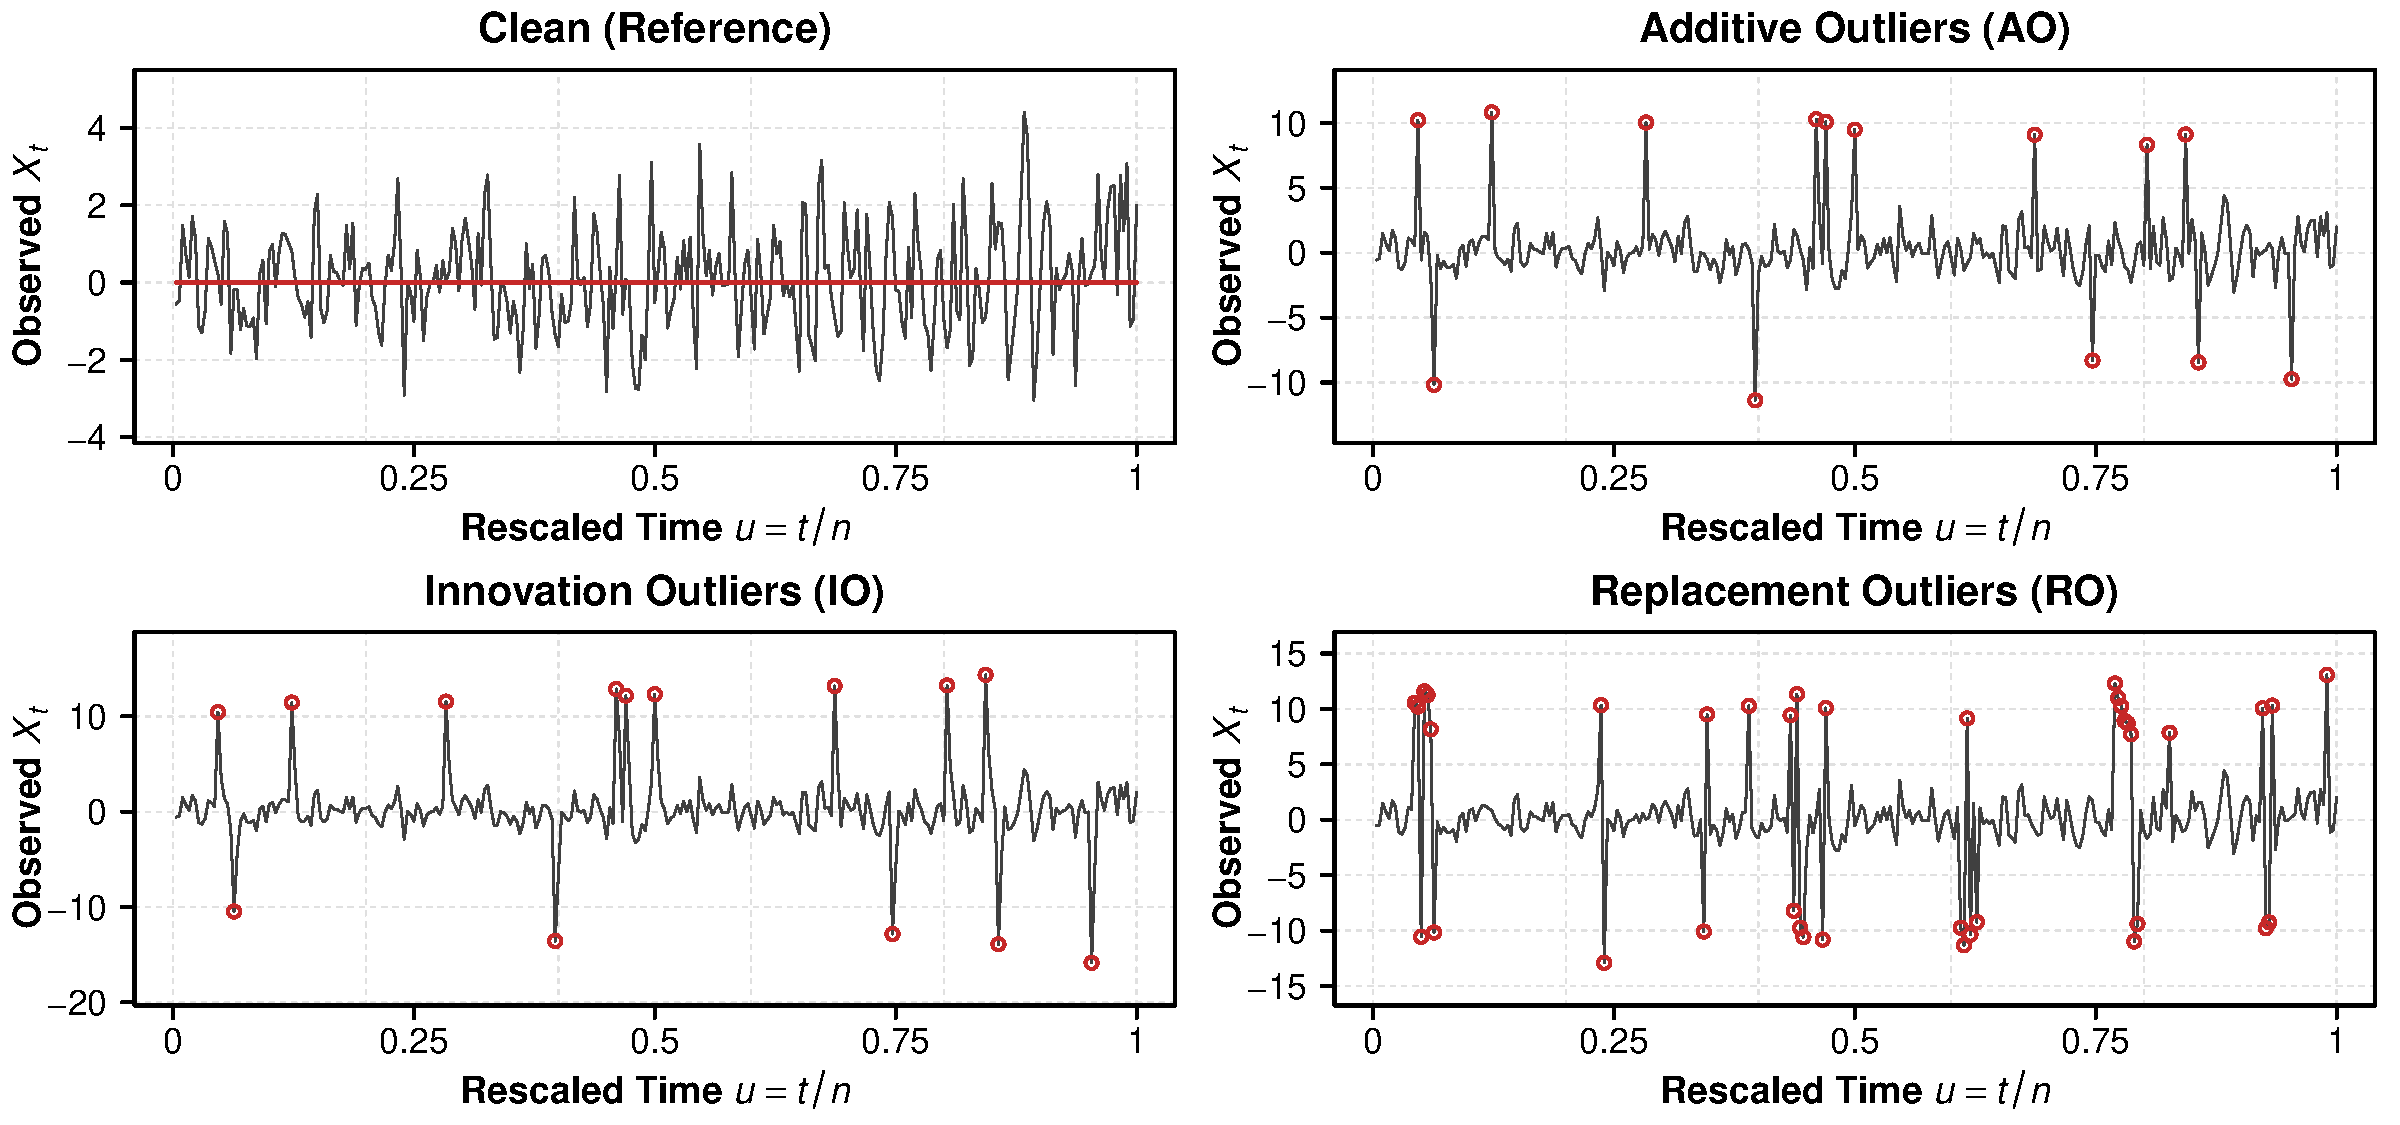
\includegraphics[width=1\linewidth]{img/X_location.pdf}
    \caption{\footnotesize \textbf{Simulated trajectories from the location DGP across contamination scenarios under an abrupt structural break ($\mathcal{H}_1$).}
    The clean baseline (top left) follows an ARMA(2,1) model with time-varying scale $\sigma(u) = \exp(u)$ and an abrupt jump $\delta = 0.50$ at $u = 0.50$; the blue solid line indicates the true theoretical expectation $m(u) = \mu(u)/(1 - a_1 - a_2)$. The remaining panels depict the three contamination mechanisms with contamination probability $\varepsilon = 0.05$ and shock magnitude $K = 10$: Additive Outliers (AO, top right), Innovation Outliers (IO, bottom left), where innovation shocks propagate through autoregressive filtering, and Replacement Outliers (RO, bottom right), where a 2-state Markov chain generates persistent contamination clusters. Red circles mark the observations affected by contamination.}
    \label{fig:X_location}
\end{figure}

\paragraph{Bandwidth Selection Strategy}
The practical implementation of our change-point framework requires specifying the local estimation bandwidth $M$. In this simulation, we use $M$ that minimizes the system of equations on an unseen future observation at lag $L_n$. Formally, the optimal bandwidth is selected by solving:
\begin{equation}
    M^{\text{opt}} = \arg\min_{M \in \mathcal{M}_n} \Lambda(M), \qquad \text{where} \quad \Lambda(M) = \sum_{t=k}^{N - L_n} \left\| H\left(X_{t+L_n,n}, \widehat{\theta}_{t}(M)\right) \right\|^2
\end{equation}
where $\mathcal{M}_n = \{ \lfloor n^{0.45}\rfloor, \lfloor n^{0.65} \rfloor \}$ defines the admissible search space ensuring asymptotic consistency, and $L_n = \lfloor \frac{1}{10} (\log n)^2 \rfloor$ denotes the decoupling lag. Although an automatic selection procedure for $L_n$ would be desirable, we adopt this choice following \cite{Mies2023}, where it demonstrated the best overall empirical performance. Finally, we set the window size for variance estimation to $b_n = L_n$.


\paragraph{Simulation Results}
We divide our numerical evaluation into two complementary analyses: first, we examine the finite-sample estimation accuracy (Mean Absolute Error and empirical Bias) of the proposed linearized recursive estimator $\widehat{\Theta}_n^{\text{lin}}(1)$ relative to the standard non-linearized plug-in estimator $\widetilde{\Theta}_n(1)$; second, we investigate the empirical size and power of our proposed CUSUM test against leading robust change-point detection procedures.

\subparagraph{Point Estimation: Bias Correction and Robustness}
Table~\ref{tab:robust_location_bias} reports the Mean Absolute Error (MAE) and empirical Bias for $\widehat{\Theta}_n^{\text{lin}}(1)$ and $\widetilde{\Theta}_n(1)$ across sample sizes $n \in \{100, 500, 1000, 5000\}$ under variance scenario (i) ($\sigma(u) = \exp(u/2)$).
Under the null hypothesis of structural stability ($\mathcal{H}_0$), both estimators perform nearly identically, exhibiting negligible bias ($< 0.002$ in magnitude for $n \ge 500$) and monotonically decaying MAE of order $O(n^{-1/2})$.

Under the alternative hypotheses ($\mathcal{H}_1$ and $\mathcal{H}_2$), however, their finite-sample behaviors diverge significantly. Because standard rolling-window M-estimation suffers from an intrinsic tracking delay across structural shifts, the non-linearized estimator $\widetilde{\Theta}_n(1)$ accumulates severe lag bias. At $n=100$, $\widetilde{\Theta}_n(1)$ exhibits a bias of $-0.047$ under Clean Gaussian data for $\mathcal{H}_1$, remaining as high as $-0.009$ even at $n=5000$. In sharp contrast, the linearized estimator $\widehat{\Theta}_n^{\text{lin}}(1)$ analytically removes this first-order bias, reducing it to $-0.008$ at $n=100$ and $0.000$ at $n=5000$, while consistently lowering the MAE across all sample sizes.

Importantly, this bias correction is fully robust to heavy-tailed innovations ($t_3$) and outlier contamination regimes. Under Innovation Outliers (IO), where shocks propagate through the autoregressive dynamics and create localized bursts of outliers, standard estimation is vulnerable to persistent tracking distortion; here, $\widehat{\Theta}_n^{\text{lin}}(1)$ achieves a major reduction in both bias (e.g., at $n=100$, $-0.003$ vs.\ $-0.058$ for $t_3$) and MAE ($0.243$ vs.\ $0.274$), illustrating the practical benefit of combining the smooth Welsh loss with analytical linearization.

\begin{table}[ht]
\centering
\caption{Mean Absolute Error (MAE) and Bias of $\widehat{\Theta}_n^{\text{lin}}(1)$ and $\widetilde{\Theta}_n(1)$ as estimators of $\int_0^1 m(u)du$ under structural breaks and data contamination. Values based on Monte Carlo replications.}
\label{tab:robust_location_bias}
\resizebox{\textwidth}{!}{
\begin{tabular}{clllcc|cc|cc|cc}
\toprule
& & & & \multicolumn{2}{c}{$n=100$} & \multicolumn{2}{c}{$n=500$} & \multicolumn{2}{c}{$n=1000$} & \multicolumn{2}{c}{$n=5000$} \\
\cmidrule(lr){5-6} \cmidrule(lr){7-8} \cmidrule(lr){9-10} \cmidrule(lr){11-12}
\textbf{Hypothesis} & \textbf{Scenario} & \textbf{Innovations} & \textbf{Metric} & $\widetilde{\Theta}_n$ & $\widehat{\Theta}_n^{\text{lin}}$ & $\widetilde{\Theta}_n$ & $\widehat{\Theta}_n^{\text{lin}}$ & $\widetilde{\Theta}_n$ & $\widehat{\Theta}_n^{\text{lin}}$ & $\widetilde{\Theta}_n$ & $\widehat{\Theta}_n^{\text{lin}}$ \\
\midrule
% --- H0 Section ---
\multirow{12}{*}{$\mathcal{H}_0 \text{ (No Shift)}$}
& \multirow{4}{*}{Clean} & \multirow{2}{*}{Gaussian} & MAE & 0.127 & 0.134 & 0.060 & 0.063 & 0.042 & 0.043 & 0.019 & 0.019 \\
& & & Bias & -0.008 & -0.006 & -0.001 & -0.001 & 0.001 & 0.001 & -0.001 & -0.000 \\
\cmidrule{3-12}
& & \multirow{2}{*}{$t_3$} & MAE & 0.164 & 0.170 & 0.073 & 0.077 & 0.056 & 0.058 & 0.025 & 0.025 \\
& & & Bias & 0.019 & 0.015 & -0.000 & 0.001 & -0.002 & -0.002 & 0.000 & 0.000 \\
\cmidrule{2-12}
& \multirow{4}{*}{AO} & \multirow{2}{*}{Gaussian} & MAE & 0.144 & 0.150 & 0.061 & 0.064 & 0.044 & 0.046 & 0.021 & 0.021 \\
& & & Bias & -0.004 & -0.002 & 0.001 & 0.001 & -0.002 & -0.002 & 0.000 & 0.000 \\
\cmidrule{3-12}
& & \multirow{2}{*}{$t_3$} & MAE & 0.194 & 0.197 & 0.084 & 0.085 & 0.063 & 0.063 & 0.027 & 0.028 \\
& & & Bias & 0.002 & -0.000 & -0.000 & -0.002 & -0.001 & -0.001 & -0.002 & -0.002 \\
\cmidrule{2-12}
& \multirow{4}{*}{IO} & \multirow{2}{*}{Gaussian} & MAE & 0.213 & 0.192 & 0.078 & 0.076 & 0.054 & 0.054 & 0.023 & 0.023 \\
& & & Bias & -0.002 & 0.001 & -0.002 & -0.000 & -0.002 & -0.003 & 0.000 & 0.000 \\
\cmidrule{3-12}
& & \multirow{2}{*}{$t_3$} & MAE & 0.274 & 0.243 & 0.111 & 0.106 & 0.077 & 0.075 & 0.030 & 0.031 \\
& & & Bias & 0.021 & 0.015 & -0.007 & -0.008 & -0.000 & 0.001 & 0.000 & 0.000 \\
\midrule
% --- H1 Section ---
\multirow{12}{*}{$\mathcal{H}_1 \text{ (Abrupt)}$}
& \multirow{4}{*}{Clean} & \multirow{2}{*}{Gaussian} & MAE & 0.140 & 0.143 & 0.066 & 0.064 & 0.047 & 0.044 & 0.022 & 0.021 \\
& & & Bias & -0.047 & -0.008 & -0.028 & -0.002 & -0.023 & -0.002 & -0.009 & 0.000 \\
\cmidrule{3-12}
& & \multirow{2}{*}{$t_3$} & MAE & 0.176 & 0.171 & 0.081 & 0.078 & 0.061 & 0.059 & 0.027 & 0.026 \\
& & & Bias & -0.057 & -0.014 & -0.031 & 0.000 & -0.027 & -0.003 & -0.013 & -0.001 \\
\cmidrule{2-12}
& \multirow{4}{*}{AO} & \multirow{2}{*}{Gaussian} & MAE & 0.153 & 0.148 & 0.066 & 0.063 & 0.050 & 0.046 & 0.023 & 0.022 \\
& & & Bias & -0.061 & -0.014 & -0.031 & -0.001 & -0.024 & -0.002 & -0.010 & 0.001 \\
\cmidrule{3-12}
& & \multirow{2}{*}{$t_3$} & MAE & 0.210 & 0.207 & 0.089 & 0.084 & 0.064 & 0.061 & 0.031 & 0.029 \\
& & & Bias & -0.061 & -0.008 & -0.034 & 0.001 & -0.022 & 0.003 & -0.014 & -0.000 \\
\cmidrule{2-12}
& \multirow{4}{*}{IO} & \multirow{2}{*}{Gaussian} & MAE & 0.216 & 0.181 & 0.082 & 0.077 & 0.061 & 0.055 & 0.027 & 0.025 \\
& & & Bias & -0.067 & -0.013 & -0.033 & 0.004 & -0.031 & -0.004 & -0.015 & -0.001 \\
\cmidrule{3-12}
& & \multirow{2}{*}{$t_3$} & MAE & 0.283 & 0.243 & 0.113 & 0.110 & 0.077 & 0.072 & 0.035 & 0.033 \\
& & & Bias & -0.058 & -0.003 & -0.032 & 0.006 & -0.028 & 0.002 & -0.015 & 0.001 \\
\midrule
% --- H2 Section ---
\multirow{12}{*}{$\mathcal{H}_2 \text{ (Gradual)}$}
& \multirow{4}{*}{Clean} & \multirow{2}{*}{Gaussian} & MAE & 0.139 & 0.143 & 0.065 & 0.061 & 0.047 & 0.044 & 0.022 & 0.020 \\
& & & Bias & -0.047 & -0.014 & -0.032 & -0.006 & -0.023 & -0.002 & -0.012 & -0.002 \\
\cmidrule{3-12}
& & \multirow{2}{*}{$t_3$} & MAE & 0.177 & 0.172 & 0.089 & 0.083 & 0.060 & 0.058 & 0.027 & 0.026 \\
& & & Bias & -0.054 & -0.020 & -0.042 & -0.014 & -0.027 & -0.003 & -0.013 & 0.001 \\
\cmidrule{2-12}
& \multirow{4}{*}{AO} & \multirow{2}{*}{Gaussian} & MAE & 0.151 & 0.151 & 0.073 & 0.069 & 0.049 & 0.046 & 0.024 & 0.021 \\
& & & Bias & -0.059 & -0.019 & -0.034 & -0.005 & -0.024 & -0.001 & -0.012 & -0.001 \\
\cmidrule{3-12}
& & \multirow{2}{*}{$t_3$} & MAE & 0.199 & 0.190 & 0.092 & 0.085 & 0.067 & 0.064 & 0.031 & 0.028 \\
& & & Bias & -0.072 & -0.026 & -0.039 & -0.007 & -0.027 & -0.001 & -0.016 & -0.002 \\
\cmidrule{2-12}
& \multirow{4}{*}{IO} & \multirow{2}{*}{Gaussian} & MAE & 0.222 & 0.187 & 0.083 & 0.078 & 0.060 & 0.055 & 0.028 & 0.024 \\
& & & Bias & -0.066 & -0.022 & -0.035 & -0.003 & -0.029 & -0.002 & -0.017 & -0.002 \\
\cmidrule{3-12}
& & \multirow{2}{*}{$t_3$} & MAE & 0.275 & 0.238 & 0.117 & 0.105 & 0.080 & 0.075 & 0.036 & 0.033 \\
& & & Bias & -0.066 & -0.026 & -0.046 & -0.011 & -0.032 & -0.005 & -0.019 & -0.003 \\
\bottomrule
\end{tabular}
}
\end{table}

\subparagraph{Change-Point Testing: Size Control and Heteroskedasticity Invariance}
We next benchmark our proposed linearized Welsh CUSUM test (\textbf{L}) against four leading robust and heteroskedasticity-aware change-point procedures:
(i) the Huber loss $M$-estimator test (\textbf{H}) of \citet{huskova2012};
(ii) the non-parametric Wilcoxon test (\textbf{W}) of \citet{Dehling2015};
(iii) the two-sample Hodges--Lehmann test (\textbf{T}) of \citet{Dehling2020}; and
(iv) the self-normalized Gini-type test (\textbf{S}) of \citet{schmidt2021}, explicitly designed to test for mean breaks under unconditional heteroskedasticity using block-based subsampling.
Figure~\ref{fig:cpd_comparison_matrix} displays the empirical rejection frequencies across sample sizes $n \in \{200, 500, 700\}$ under the nominal significance level $\alpha = 0.05$.

The empirical size results under $\mathcal{H}_0$ (first column of Figure~\ref{fig:cpd_comparison_matrix}) reveal a sharp demarcation between robustness to outlier shocks and robustness to non-stationary volatility. Under smooth trending variance (case~(i), blue circles), all tests maintain reasonable size control close to the nominal $5\%$ level. However, when subjected to cyclic heteroskedasticity (case~(ii), green circles) or an abrupt variance break (case~(iii), red circles), classical robust benchmark methods exhibit severe distortions:
\begin{itemize}
    \item The two-sample Hodges--Lehmann test (\textbf{T}) experiences a catastrophic size collapse under cyclic variance, falsely rejecting the null in over $60\%$ of replications (reaching $73.8\%$ at $n=700$ for clean Gaussian series). These points exceed the $0.25$ plotting ceiling and are off-scale. Under the variance break (case~(iii)), its false rejection rate also inflates to $11.6\% - 14.2\%$. Because two-sample rank statistics evaluate pairwise differences $X_j - X_i$ between sub-samples, asymmetric dispersion between the first and second halves of the series fundamentally distorts the rank distribution, which the test misinterprets as a location shift.
    \item The Wilcoxon test (\textbf{W}) similarly shows marked size inflation under cyclic variance, rejecting up to $10.4\%$ under the null.
    \item The Huberized CUSUM (\textbf{H}) displays greater resilience than rank-based methods, keeping empirical size between $4.6\%$ and $9.2\%$. Because Huber's score $\psi_c(\cdot)$ is an odd function, $\mathbb{E}[\psi_c(X_t/\sigma(u))] = 0$ holds pointwise for symmetric distributions, preventing spurious mean drift. Nevertheless, because \textbf{H} studentizes using a single global long-run variance estimator that assumes stationarity, cyclic volatility still causes non-negligible size inflation.
    \item The Gini-based test (\textbf{S}) of \citet{schmidt2021} successfully accommodates unconditional heteroskedasticity through its block-based subsampling variance estimator, maintaining stable size under smooth trending and cyclic variance. However, because it operates directly on raw block averages without robust bounded score functions, its finite-sample calibration degrades in the presence of heavy-tailed innovations and clustered replacement outliers.
    \item In sharp contrast, our proposed linearized test (\textbf{L}) is the \textbf{only method in the study that achieves complete invariance to heteroskedasticity}. Across all three variance scenarios, its average empirical size remains tightly anchored around the nominal level: $5.7\%$ for case~(i), $5.9\%$ for case~(ii), and $5.8\%$ for case~(iii). By integrating local non-parametric variance estimation with boundary decoupling at lag $L_n$, \textbf{L} standardizes the partial sums dynamically, guaranteeing that volatility shifts are never conflated with breaks in location.
\end{itemize}

\subparagraph{Power Evaluation under Abrupt and Gradual Shifts}
Columns 2 and 3 of Figure~\ref{fig:cpd_comparison_matrix} report empirical power under abrupt ($\mathcal{H}_1$) and gradual ($\mathcal{H}_2$) location changes with shift magnitude $\delta = 0.5$. In comparing power, we focus on baseline environments where tests maintain valid size control (case~(i)), since the high rejection rates of test \textbf{T} under cyclic heteroskedasticity are spurious artifacts of its $63\%$ false alarm rate.

Under $\mathcal{H}_1$ (abrupt break at $u=0.5$), detection power increases rapidly toward $1.0$ as $n$ grows from $200$ to $700$ ($0.434 \to 0.832$ for \textbf{L}). In case~(i), the power of our proposed method ($0.598$) closely matches that of the Huberized CUSUM ($0.592$) and rank-based tests ($0.626$ for \textbf{W}, $0.634$ for \textbf{T}), demonstrating that the heteroskedasticity robustness of \textbf{L} incurs no power penalty under well-behaved stationary volatility.

Under $\mathcal{H}_2$ (gradual linear change), the location change accumulates smoothly throughout the horizon, making the break more difficult to identify locally. Nonetheless, power increases monotonically with $n$ across all configurations. Furthermore, under Innovation Outliers (IO) and Replacement Outliers (RO), where shocks propagate or persistently overwrite observations, the smooth exponential downweighting of the Welsh loss $\psi(u) = u \exp(-(u/c)^2)$ prevents contamination bursts from destabilizing the CUSUM path, yielding superior stability and power progression over competing rank and block-based tests.

\begin{figure}[h!]
    \centering
    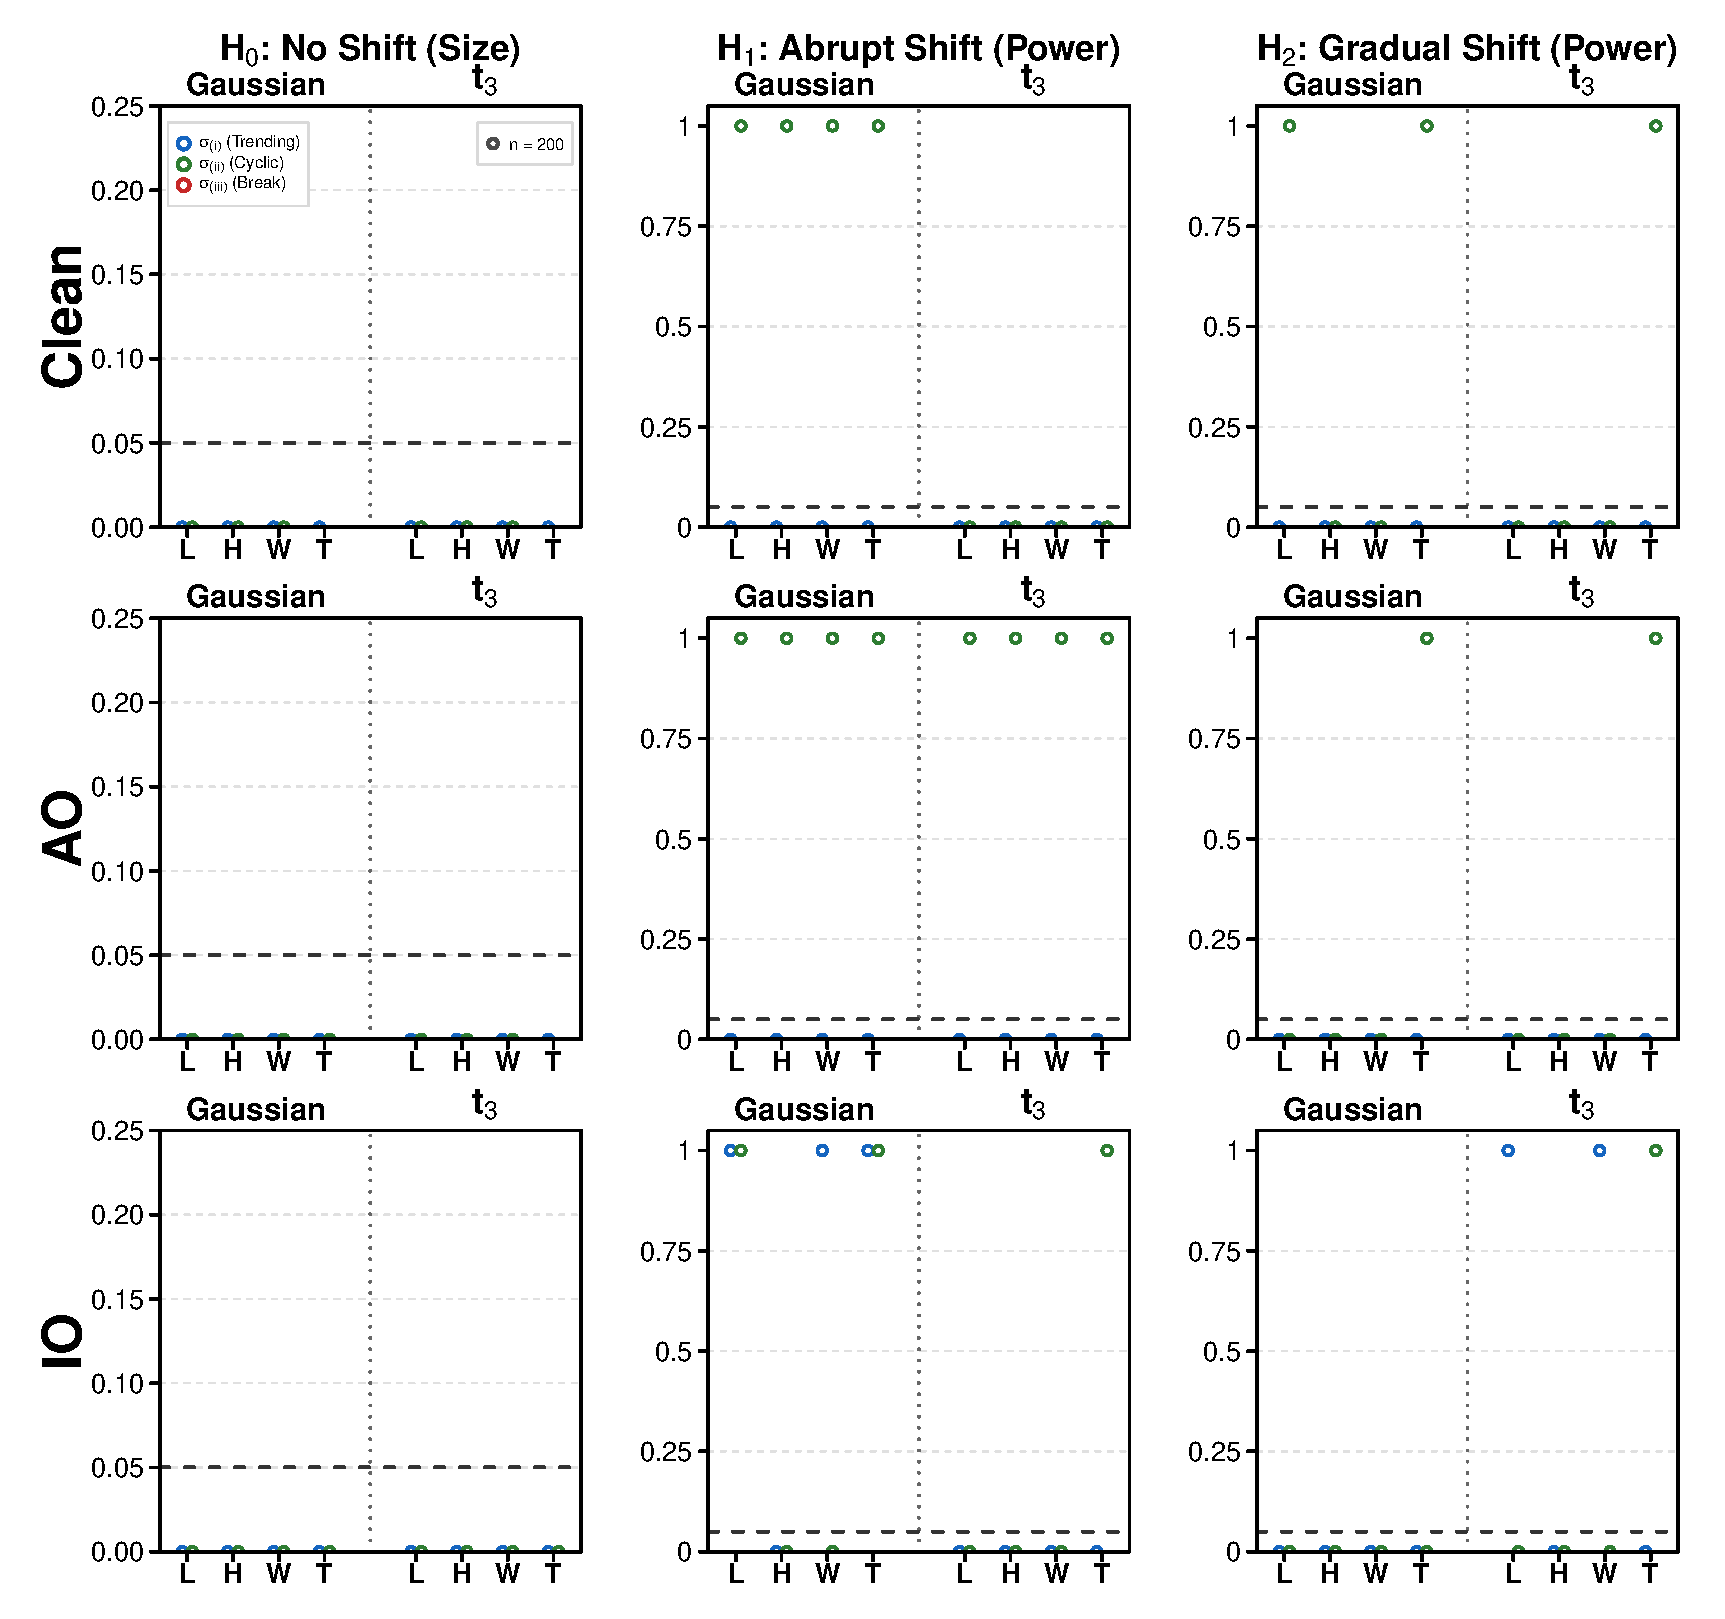
\includegraphics[width=1\textwidth]{img/cpd_comparison_matrix.pdf}
    \caption{\footnotesize \textbf{Empirical rejection rates for robust location change-point tests under ARMA(2,1) dependence.}
    Evaluated under $H_0$ (size), $H_1$ (abrupt break at $u=0.5$), and $H_2$ (gradual linear change) with shift magnitude $\delta = 0.5$ at nominal level $\alpha = 0.05$ (dashed line). Rows represent Clean, AO, IO, and RO with $\varepsilon = 0.05$ scenarios for Gaussian and Student-$t_3$ errors. Methods: \textbf{L} (Proposed Linearized Welsch CUSUM), \textbf{H} (Huberized CUSUM; \cite{huskova2012}), \textbf{W} (Wilcoxon test; \cite{Dehling2015}), \textbf{T} (Hodges--Lehmann test; \cite{Dehling2020}), and \textbf{S} (Schmidt's Gini test; \cite{schmidt2021}). Circle colors represent variance scenarios: smooth trending (blue), cyclic (green), and abrupt break (red). Open circle markers scale with sample size $n \in \{200, 500, 700\}$.}
    \label{fig:cpd_comparison_matrix}
\end{figure}



% \begin{table}[ht]
% \centering
% \caption{Mean Square Error and Bias of $\widehat{\Theta}_n^{\text{lin}}(1)$ and $\widetilde{\Theta}_n(1)$ as estimators of $\int_0^1 m(u)du$ under structural breaks and data contamination with $\varepsilon = 0.10$. Values based on 1000 Monte Carlo replications.}
% \label{tab:robust_location_bias}
% \resizebox{\textwidth}{!}{
% \begin{tabular}{clllcc|cc|cc|cc}
% \toprule
% & & & & \multicolumn{2}{c}{$n=100$} & \multicolumn{2}{c}{$n=500$} & \multicolumn{2}{c}{$n=1000$} & \multicolumn{2}{c}{$n=5000$} \\
% \cmidrule(lr){5-6} \cmidrule(lr){7-8} \cmidrule(lr){9-10} \cmidrule(lr){11-12}
% \textbf{Hypothesis} & \textbf{Scenario} & \textbf{Innovations} & \textbf{Metric} & $\widetilde{\Theta}_n$ & $\widehat{\Theta}_n^{\text{lin}}$ & $\widetilde{\Theta}_n$ & $\widehat{\Theta}_n^{\text{lin}}$ & $\widetilde{\Theta}_n$ & $\widehat{\Theta}_n^{\text{lin}}$ & $\widetilde{\Theta}_n$ & $\widehat{\Theta}_n^{\text{lin}}$ \\
% \midrule
% % --- H0 Section ---
% \multirow{12}{*}{$\mathcal{H}_0 \text{ (No Shift)}$}
% & \multirow{4}{*}{Clean} & \multirow{2}{*}{Gaussian} & Error & 0.014 & 0.015 & 0.003 & 0.003 & 0.002 & 0.002 & 0.000 & 0.000 \\
% & & & Bias & 0.003 & 0.001 & 0.001 & 0.001 & 0.000 & 0.001 & 0.001 & 0.001 \\
% \cmidrule{3-12}
% & & \multirow{2}{*}{$t_3$} & Error & 0.023 & 0.025 & 0.005 & 0.005 & 0.003 & 0.003 & 0.001 & 0.001 \\
% & & & Bias & -0.011 & -0.008 & 0.005 & 0.005 & 0.000 & 0.000 & -0.000 & -0.000 \\
% \cmidrule{2-12}
% & \multirow{4}{*}{AO} & \multirow{2}{*}{Gaussian} & Error & 0.014 & 0.015 & 0.003 & 0.003 & 0.002 & 0.002 & 0.000 & 0.000 \\
% & & & Bias & 0.000 & 0.003 & -0.001 & -0.002 & -0.000 & -0.000 & 0.001 & 0.002 \\
% \cmidrule{3-12}
% & & \multirow{2}{*}{$t_3$} & Error & 0.021 & 0.024 & 0.005 & 0.006 & 0.003 & 0.003 & 0.001 & 0.001 \\
% & & & Bias & 0.005 & 0.004 & 0.002 & 0.000 & -0.002 & -0.002 & -0.001 & -0.000 \\
% \cmidrule{2-12}
% & \multirow{4}{*}{IO} & \multirow{2}{*}{Gaussian} & Error & 0.016 & 0.017 & 0.004 & 0.004 & 0.002 & 0.002 & 0.000 & 0.000 \\
% & & & Bias & 0.004 & 0.006 & 0.000 & 0.001 & 0.000 & 0.000 & 0.000 & -0.000 \\
% \cmidrule{3-12}
% & & \multirow{2}{*}{$t_3$} & Error & 0.027 & 0.034 & 0.006 & 0.007 & 0.003 & 0.003 & 0.001 & 0.001 \\
% & & & Bias & 0.001 & 0.001 & 0.001 & -0.001 & -0.002 & -0.002 & 0.002 & 0.002 \\
% \midrule
% % --- H1 Section ---
% \multirow{12}{*}{$\mathcal{H}_1 \text{ (Abrupt)}$}
% & \multirow{4}{*}{Clean} & \multirow{2}{*}{Gaussian} & Error & 0.052 & 0.018 & 0.019 & 0.003 & 0.011 & 0.002 & 0.003 & 0.000 \\
% & & & Bias & -0.192 & -0.016 & -0.126 & -0.008 & -0.097 & -0.001 & -0.056 & -0.001 \\
% \cmidrule{3-12}
% & & \multirow{2}{*}{$t_3$} & Error & 0.067 & 0.032 & 0.020 & 0.006 & 0.012 & 0.003 & 0.004 & 0.001 \\
% & & & Bias & -0.208 & -0.029 & -0.123 & -0.004 & -0.097 & -0.001 & -0.056 & -0.001 \\
% \cmidrule{2-12}
% & \multirow{4}{*}{AO} & \multirow{2}{*}{Gaussian} & Error & 0.057 & 0.021 & 0.018 & 0.004 & 0.012 & 0.002 & 0.004 & 0.000 \\
% & & & Bias & -0.200 & -0.020 & -0.120 & -0.002 & -0.100 & -0.003 & -0.057 & -0.001 \\
% \cmidrule{3-12}
% & & \multirow{2}{*}{$t_3$} & Error & 0.069 & 0.033 & 0.021 & 0.006 & 0.012 & 0.003 & 0.004 & 0.001 \\
% & & & Bias & -0.208 & -0.024 & -0.125 & -0.005 & -0.099 & -0.004 & -0.056 & -0.001 \\
% \cmidrule{2-12}
% & \multirow{4}{*}{IO} & \multirow{2}{*}{Gaussian} & Error & 0.058 & 0.022 & 0.019 & 0.004 & 0.011 & 0.002 & 0.004 & 0.000 \\
% & & & Bias & -0.202 & -0.023 & -0.124 & -0.005 & -0.097 & -0.000 & -0.057 & -0.002 \\
% \cmidrule{3-12}
% & & \multirow{2}{*}{$t_3$} & Error & 0.065 & 0.037 & 0.022 & 0.007 & 0.013 & 0.003 & 0.004 & 0.001 \\
% & & & Bias & -0.190 & -0.012 & -0.125 & -0.005 & -0.100 & -0.005 & -0.055 & 0.000 \\
% \midrule
% % --- H2 Section ---
% \multirow{12}{*}{$\mathcal{H}_2 \text{ (Gradual)}$}
% & \multirow{4}{*}{Clean} & \multirow{2}{*}{Gaussian} & Error & 0.056 & 0.018 & 0.019 & 0.004 & 0.011 & 0.002 & 0.003 & 0.000 \\
% & & & Bias & -0.206 & -0.060 & -0.124 & -0.019 & -0.095 & -0.008 & -0.056 & -0.003 \\
% \cmidrule{3-12}
% & & \multirow{2}{*}{$t_3$} & Error & 0.063 & 0.028 & 0.020 & 0.005 & 0.012 & 0.003 & 0.004 & 0.001 \\
% & & & Bias & -0.201 & -0.052 & -0.121 & -0.015 & -0.099 & -0.011 & -0.057 & -0.003 \\
% \cmidrule{2-12}
% & \multirow{4}{*}{AO} & \multirow{2}{*}{Gaussian} & Error & 0.055 & 0.019 & 0.018 & 0.004 & 0.011 & 0.002 & 0.003 & 0.000 \\
% & & & Bias & -0.201 & -0.052 & -0.123 & -0.017 & -0.098 & -0.010 & -0.055 & -0.002 \\
% \cmidrule{3-12}
% & & \multirow{2}{*}{$t_3$} & Error & 0.066 & 0.030 & 0.020 & 0.006 & 0.012 & 0.003 & 0.004 & 0.001 \\
% & & & Bias & -0.204 & -0.054 & -0.122 & -0.017 & -0.097 & -0.010 & -0.055 & -0.003 \\
% \cmidrule{2-12}
% & \multirow{4}{*}{IO} & \multirow{2}{*}{Gaussian} & Error & 0.059 & 0.021 & 0.019 & 0.004 & 0.011 & 0.002 & 0.003 & 0.000 \\
% & & & Bias & -0.205 & -0.057 & -0.126 & -0.019 & -0.097 & -0.010 & -0.055 & -0.002 \\
% \cmidrule{3-12}
% & & \multirow{2}{*}{$t_3$} & Error & 0.068 & 0.068 & 0.022 & 0.007 & 0.013 & 0.003 & 0.004 & 0.001 \\
% & & & Bias & -0.201 & -0.046 & -0.126 & -0.020 & -0.097 & -0.009 & -0.056 & -0.003 \\
% \bottomrule

% \end{tabular}
% }
% \end{table}


\newpage
\subsection{Time-Varying Robust M-Regression}

In this section, we examine the finite-sample performance of the proposed CUSUM test for the robust time-varying regression model introduced in Example \ref{ex:robtv}. 
Let $D_{t,n} = (X_{t,n}^\top, Y_{t,n})^\top \in \mathbb{R}^{d+1}$, for $t = 1, \dots, n$, be a triangular array of observations governed by the causal locally stationary data-generating mechanism
\begin{equation}
    Y_{t,n} = X_{t,n}^\top \beta\left(\frac{t}{n}\right) + \nu_{t,n}, \quad t = 1, \dots, n,
\end{equation}
where $X_{t,n} \in \mathbb{R}^d$ is a vector of locally stationary regressors, $\beta(u) = (\beta_1(u), \dots, \beta_d(u))^\top \in \mathcal{C}^2([0, 1], \mathbb{R}^d)$ represents the vector of time-varying regression coefficients, and $\nu_{t,n}$ is a process satisfying the moment condition $\mathbb{E}[\psi(Y_{t,n} - X_{t,n}^\top \beta(t/n)) \mid \mathcal{F}_{t-1}, X_{t,n}] = 0$ almost surely, with $\psi(\cdot)$ being a robust score function $\in \mathcal{C}^2([0, 1]) $.

We are interested in testing whether the regression parameters are structurally stable over the observation horizon, let $\mathbf{C} \in \mathbb{R}^{s\times d}$ be the selection matrix with rank $\{s \le d\}$ we want to test:
\begin{equation*}
    \mathcal{H}_0: \mathbf{C}\beta(u) \equiv \beta_C \quad \text{for all } u \in [0, 1] \quad \text{vs.} \quad \mathcal{H}_1: \beta(u) \not\equiv \beta_C \quad \text{for some } u \in [0, 1].
\end{equation*}

\paragraph{Simulation Data Generating Processes}
To assess both size control under non-stationary nuisance dynamics and power against structural changes, we generate observations under two distinct specifications.

We first introduce the building blocks of the data-generating mechanisms. Let $u = t/n \in [0, 1]$ denote the normalized time index. We define the bivariate covariate process $X_{t,n} = (x^1_{t,n}, x^2_{t,n})^\top \in \mathbb{R}^2$, where each component $x^i_{t,n}$ is represented as a time-varying linear filter of the past innovation shocks $\{\epsilon_{i,t}\}_{t=-\infty}^\infty$ for $i \in \{1, 2\}$:
\begin{equation*}
    x^i_{t,n} = \sum_{j=0}^\infty \left[\phi_i\left(\frac{t}{n}\right)\right]^j \epsilon_{i,t-j}, \quad i \in \{1, 2\},
\end{equation*}
where the geometric decay functions satisfy $\sup_{u \in [0, 1]} |\phi_i(u)| < 1$ to guarantee short-range dependence and uniform ergodicity. Specifically, we calibrate the time-varying memory via $\phi_1(u) = 0.5 - 0.5u$ and $\phi_2(u) = 0.25 + 0.5u$. The innovation sequences $\{\epsilon_{1,t}\}$ and $\{\epsilon_{2,t}\}$ consist of independent standard normal random variables.

The baseline error sequence $e_{t,n}$ is generated from innovation shocks $\{\eta_t\}_{t=-\infty}^\infty$:
\begin{equation*}
    e_{t,n} = \sum_{j=0}^\infty \left[\xi\left(\frac{t}{n}\right)\right]^j \eta_{t-j},
\end{equation*}
with time-varying persistence $\xi(u) = 0.5 - (u - 0.5)^2 \in [0.25, 0.5]$. The innovations $\eta_t$ are drawn either from a standard Gaussian distribution $\mathcal{N}(0, 1)$ or a heavy-tailed Student's $t_3$ distribution.

We consider the following two models:

\begin{enumerate}[label=(\roman*)]
    \item \textbf{Model I: Linear Model with Conditional Heteroscedasticity (LMCH).}
    \begin{equation}
    \label{eq: model1reg}
        Y_{t,n} = X_{t,n}^\top \beta\left(\frac{t}{n}\right) + \Gamma(X_{t,n}) \, e_{t,n},
    \end{equation}
    where the conditional scale function induces severe regressor-dependent heteroscedasticity via
    \begin{equation*}
        \Gamma(X_{t,n}) = \sqrt{1 + \|X_{t,n}\|_2^2} = \sqrt{1 + (x^1_{t,n})^2 + (x^2_{t,n})^2}.
    \end{equation*}
    Because $\mathbb{E}[e_{t,n} \mid X_{t,n}] = 0$, the conditional moment condition $\mathbb{E}[\psi(Y_{t,n} - X_{t,n}^\top \beta(t/n)) \mid X_{t,n}] = 0$ holds exactly, while the noise variance $\operatorname{Var}(\nu_{t,n} \mid X_{t,n}) = \Gamma(X_{t,n})^2 \operatorname{Var}(e_{t,n})$ fluctuates substantially with the covariate paths, rigorously challenging the robustness of the variance estimator.

    \item \textbf{Model II:  Linear Model with Unconditional Heteroscedasticit (LMUH).}
    \begin{equation}
    \label{eq: model2reg}
        Y_{t,n} = X_{t,n}^\top \beta\left(\frac{t}{n}\right) + \sigma\left(\frac{t}{n}\right) e_{t,n},
    \end{equation}

    Where the deterministic volatility trend is given by $\sigma(u) = 0.5 + |\sin(2\pi u)|$, and the innovation process $e_{t,n}$ is conditionally independent of $X_{t,n}$.
\end{enumerate}

\paragraph{Target Parameter and Hypotheses}
To evaluate both the size control under the null hypothesis and the sensitivity of the proposed test against structural instability, we test the constancy of the regression parameters against two canonical departure mechanisms parameterized by a perturbation scalar $\delta \ge 0$. Following the benchmark designs in \citet{zhang2012}, \citet{Mies2023} and \citet{liu2024}, we focus on an isolated regime break and a continuous macroscopic trend:
\begin{align*}
    \mathcal{H}_0: \quad & \beta(u) =  \beta_0 \\
    \mathcal{H}_1: \quad & \beta(u) = \beta_0 + \delta \, \mathbf{v} \, \mathbf{1}_{\{u > 0.5\}}, \quad u \in [0, 1] 
     \quad \text{(Abrupt Shift)} \\
    \mathcal{H}_2: \quad & \beta(u) = \beta_0 + \delta \, \mathbf{v} \, u, \quad u \in [0, 1] \quad \text{(Gradual Shift)}
\end{align*}

    where $\mathbf{1}_{\{\cdot\}}$ is the indicator function and $\mathbf{v} \in \mathbb{R}^d$ is a directional contrast vector that dictates which coefficient undergoes structural transition. For Model~I (LMHC), we set $\beta_0 = (1.0, 2.0)^\top$ and perturb the primary exogenous covariate by choosing $\mathbf{v} = (1, 0)^\top$. For Model~II (LMAT), where the stacked baseline parameter is $\beta_0 = (0.4, 1.0, 0.5)^\top$, we perturb the first exogenous predictor using $\mathbf{v} = (0, 1, 0)^\top$, keeping the autoregressive parameter fixed at $\beta_{\text{AR}} = 0.4$ to guarantee causal stability across the entire horizon.



\paragraph{Contamination Scenarios} 
To investigate the finite-sample robustness of our proposed CUSUM test against both isolated anomalies and structural contamination, we subject the Data Generating Processes (DGPs) in \eqref{eq: model1reg} and \eqref{eq: model2reg} to three distinct outlier regimes. Throughout, let $\varepsilon =0.05$ denote the nominal contamination rate, $I_t^\varepsilon \overset{\text{i.i.d.}}{\sim} \text{Bernoulli}(\varepsilon)$ be the contamination indicator, $K = 10$ represent the shock magnitude, and $\xi_t \overset{\text{i.i.d.}}{\sim} \text{Bernoulli}(0.5)$ be independent sign-assignment variables such that $(-1)^{\xi_t} \in \{-1, 1\}$.
  
\begin{enumerate}[label=(\roman*)]
    \item \textbf{Scenario 1: Additive Outliers (AO).} 
      We generate additive outliers in the predictor response $Y_{t,n}$ via:
    \begin{align*}
        Y_{t,n}^{\text{AO}} &= Y_{t,n} + I_t^\varepsilon \, (-1)^{\xi_t} K, 
    \end{align*}
     Because the true latent path is uncorrupted, the shock at time $t$ does not propagate into future time periods.

    \item \textbf{Scenario 2: Innovation Outliers (IO).} 
    We contaminate the baseline white noise $\eta_t$ driving $e_{t,n}$ prior to filtering:
    \begin{equation*}
        \eta_t^{\text{IO}} = \eta_t + I_t^\varepsilon \, (-1)^{\xi_t} K,
    \end{equation*}
   The contaminated error process $e_{t,n}^{\text{IO}} = \sum_{j=0}^\infty [\xi(t/n)]^j \eta_{t-j}^{\text{IO}}$ dynamically inherits the memory of past contamination shocks, producing localized outlier clusters that challenge standard non-robust variance estimation.

    \item \textbf{Scenario 3: Replacement Outliers (RO).} 
While AO and IO have already been discussed in Section~\ref{sec:simulation_robust_location}, here we introduce an additional contamination scenario based on replacement. Under this scheme, the observed response variable $Y_{t,n}^{\text{RO}}$ is generated by completely overwriting the latent clean process $Y_{t,n}$ during contaminated periods:
\begin{equation*}
    Y_{t,n}^{\text{RO}} = (1 - \delta_t) Y_{t,n} + \delta_t Y^*_{t,n},
\end{equation*}
where $Y^*_{t,n}$ denotes an independent contaminating replacement process and $\delta_t \in \{0, 1\}$ is a binary switching indicator with marginal contamination probability $\mathbb{P}(\delta_t = 1) = \varepsilon$. Notice that standard additive contamination can be recovered as a degenerate special case where $Y^*_{t,n} = Y_{t,n} + (-1)^\xi K$. 

Crucially, the replacement framework allows us to simulate more realistic and challenging patch (or burst) outliers by modeling $\delta_t$ via a two-state Markov chain $S_t \in \{0, 1\}$. Let $S_t = 1$ denote the active replacement regime and $S_t = 0$ denote the clean baseline regime. To calibrate the stationary marginal contamination probability to $\mathbb{P}(S_t = 1) = \varepsilon$ and the recovery probability to $\mathbb{P}(S_t = 0 \mid S_{t-1} = 1) = \kappa \in (0, 1)$, detailed balance requires the contamination onset probability to satisfy:
\begin{equation*}
    \mathbb{P}(S_t = 1 \mid S_{t-1} = 0) = \frac{\mathbb{P}(S_{t-1} = 1) \, \mathbb{P}(S_t = 0 \mid S_{t-1} = 1)}{\mathbb{P}(S_{t-1} = 0)} = \frac{\kappa \varepsilon}{1 - \varepsilon}.
\end{equation*}
During contaminated periods ($S_t = 1$), the clean observation is overwritten using
\begin{align*} 
Y^*_{t,n} &= X_{t,n}^\top \Big(\gamma \, \beta\left(\frac{t}{n}\right)\Big) + \Gamma(X_{t,n}) \, e_{t,n} \qquad \text{For Model I (LMHC)} \\
 Y^*_{t,n} &= W_{t,n}^\top \Big(\gamma \, \beta\left(\frac{t}{n}\right)\Big) + \sigma\left(\frac{t}{n}\right) e_{t,n} \qquad \text{For Model II (LMAT)}
\end{align*}
This design induces localized patches of outliers that test the resistance of the local M-estimating function when the location is not random as in the AO scenario.
\end{enumerate}
\begin{figure}
    \centering
    
\includegraphics[width=1\linewidth]{img/Y_regression.png}
    \caption{Caption}
    \label{fig:placeholder}
\end{figure}
\paragraph{Implementation Details and Bandwidth Selection}
We evaluate the finite-sample performance of the proposed linearized recursive CUSUM test across $N_{\text{sim}} = 1{,}000$ independent Monte Carlo replications for sample sizes $n \in \{500, 1{,}000, 5{,}000\}$ under a nominal significance level $\alpha = 0.05$. The multiplier bootstrap approximations are conducted using $B = 100$ bootstrap draws per replication. For the alternative departure mechanisms under $\mathcal{H}_1$ and $\mathcal{H}_2$, the perturbation magnitude is set to $\delta = \{0,0.25,0.5,0.75,1,1.25\}$


\paragraph{Results}
We compare the performance of the CUSUM test using the proposed linearized M-estimator with both Welsch and squared loss functions. The squared loss, $\rho(r) = \frac{1}{2}r^2$, corresponds to the non-robust CUSUM procedure introduced in \citet{Mies2023}. Throughout, we fix the Welsch tuning parameter to $c = 2.985$ to guarantee $95\%$ asymptotic relative efficiency under Gaussian innovations, whereas for the selection of $M$, $L_n$, and $b_n$, we follow the smae procedure used in Section~\ref{sec:simulation_robust_location}. Table~\ref{tab:empirical_size_lmhc} summarizes the empirical rejection frequencies under the null hypothesis $\mathcal{H}_0$ at the nominal level $\alpha = 0.05$. In general, the test based on the $L_2$ loss is notably conservative, which is consistent with the findings in \citet{Mies2023}. Interestingly, even in the clean setting with Gaussian innovations, the Welsch loss maintains an empirical size closer to the nominal level, despite a slight upward distortion of roughly $0.02$, whereas the $L_2$ loss yields an empirical size of only $0.011$. Moreover, under the IO scenario, both estimators become more conservative.We next analyze empirical power. Figures~\ref{fig:power_curves_matrix_gaussian} and \ref{fig:power_curves_matrix_t3} display the power curves for standard normal and $t_3$ innovations, respectively, under both alternative specifications. In the clean scenario across both figures, both loss functions exhibit comparable performance; however, the Welsch loss attains higher power earlier, detecting smaller jump sizes $\delta$. In contaminated settings, the performance of the $L_2$ loss deteriorates substantially—most noticeably under IO contamination, where the test suffers from low power even when $n = 5000$. While these contaminated setups naturally favor robust methods, the proposed M-estimation framework systematically enhances detection performance across the board.



\begin{figure}
    \centering
    
\includegraphics[width=1\linewidth]{img/power_curves_matrix_gaussian.pdf}
    \caption{\footnotesize\textbf{Empirical power curves for robust regression change-point tests under Gaussian noise.}
    Rejection rates against shift magnitude $\delta \in [0, 1.25]$ under Abrupt ($H_1$, top) and Gradual ($H_2$, bottom) structural breaks across Clean, AO, IO, and RO contamination scenarios ($\varepsilon = 0.05$). Solid lines ($\psi$) show the proposed Linearized Robust M-test with Welsch loss; dashed lines ($L_2$) show the classical non-robust CUSUM test. Colors indicate $n \in \{500, 1000, 5000\}$ ($N^{sim} = 1{,}000$ replications, $B=100$ bootstrap sample, nominal level $\alpha = 0.05$).}
    \label{fig:power_matrix_gaussian}
\end{figure}
\begin{figure}
    \centering
    
\includegraphics[width=1\linewidth]{img/power_curves_matrix_t3.pdf}
     \caption{\footnotesize\textbf{Empirical power curves for robust regression change-point tests under $t_3$ noise.}
    Rejection rates against shift magnitude $\delta \in [0, 1.25]$ under Abrupt ($H_1$, top) and Gradual ($H_2$, bottom) structural breaks across Clean, AO, IO, and RO contamination scenarios ($\varepsilon = 0.05$). Solid lines ($\psi$) show the proposed Linearized Robust M-test with Welsch loss; dashed lines ($L_2$) show the classical non-robust CUSUM test. Colors indicate $n \in \{500, 1000, 5000\}$ ($N^{sim} = 1{,}000$ replications, $B=100$ bootstrap sample, nominal level $\alpha = 0.05$).}
    \label{fig:power_curves_matrix_t3}
\end{figure}

% ==============================================================================
% Table: Empirical Size Rejection Frequencies under H0 (alpha = 0.05)
% Model: Model I (LMHC), Contamination: eps = 0.05 (alongside Clean eps = 0.00)
% ==============================================================================
\begin{table}[!htbp]
\centering
\caption{\footnotesize Empirical size rejection frequencies under the null hypothesis $\mathcal{H}_0$ (nominal level $\alpha = 0.05$) across $N_{\text{sim}} = 1{,}000$ Monte Carlo replications for sample sizes $n \in \{500, 1{,}000, 5{,}000\}$ under Model I (LMHC). }
\label{tab:empirical_size_lmhc}
\resizebox{\textwidth}{!}{%
\begin{tabular}{lllcccccccc}
\toprule
& & & & \multicolumn{3}{c}{\textbf{ Linearized M-Test}} & & \multicolumn{3}{c}{\textbf{Linearized $L_2$ Test}} \\
\cmidrule{5-7} \cmidrule{9-11}
\textbf{Model} & \textbf{Noise} & \textbf{Regime} & $\boldsymbol{\varepsilon}$ & $n = 500$ & $n = 1000$ & $n = 5000$ & & $n = 500$ & $n = 1000$ & $n = 5000$ \\
\midrule
\multirow{8}{*}{\textbf{Model I (LMHC)}}
& $\mathcal{N}(0, 1)$  & Clean & 0.00 & 0.079 & 0.075 & 0.067 & & 0.012 & 0.012 & 0.011 \\
&                      & AO    & 0.05 & 0.067 & 0.074 & 0.065 & & 0.004 & 0.008 & 0.011 \\
&                      & IO    & 0.05 & 0.020 & 0.021 & 0.028 & & 0.007 & 0.009 & 0.018 \\
&                      & RO    & 0.05 & 0.077 & 0.054 & 0.071 & & 0.016 & 0.010 & 0.028 \\
\cmidrule{2-11}
& $t_3$                & Clean & 0.00 & 0.061 & 0.062 & 0.068 & & 0.013 & 0.011 & 0.025 \\
&                      & AO    & 0.05 & 0.047 & 0.052 & 0.057 & & 0.002 & 0.006 & 0.014 \\
&                      & IO    & 0.05 & 0.014 & 0.012 & 0.026 & & 0.007 & 0.009 & 0.024 \\
&                      & RO    & 0.05 & 0.050 & 0.058 & 0.058 & & 0.010 & 0.019 & 0.022 \\
\bottomrule
\end{tabular}%
}
\end{table}



% \begin{table}[!htbp]
% \centering
% \caption{Empirical size rejection frequencies under the null hypothesis $\mathcal{H}_0$ ($\alpha = 0.05$) across $N_{\text{sim}} = 1{,}000$ Monte Carlo replications for sample sizes $n \in \{500, 1{,}000, 5{,}000\}$. The proposed Linearized Robust M-Test is compared against the Classical $L_2$/OLS CUSUM test and the Self-Convolved Bootstrap (SCB) test of \citet{liu2024} across clean, Additive Outliers (AO), Innovation Outliers (IO), and Replacement Outliers (RO) regimes.}
% \label{tab:empirical_size}
% \vspace{0.2cm}
% \resizebox{\textwidth}{!}{%
% \begin{tabular}{lllccccccccccc}
% \toprule
% & & & \multicolumn{3}{c}{\textbf{Proposed Linearized M-Test}} & & \multicolumn{3}{c}{\textbf{Classical $L_2$/OLS Test}} & & \multicolumn{3}{c}{\textbf{SCB Test \citep{liu2024}}} \\
% \cmidrule{4-6} \cmidrule{8-10} \cmidrule{12-14}
% \textbf{Model} & \textbf{Noise} & \textbf{Regime} & $n = 500$ & $n = 1000$ & $n = 5000$ & & $n = 500$ & $n = 1000$ & $n = 5000$ & & $n = 500$ & $n = 1000$ & $n = 5000$ \\
% \midrule
% \multirow{8}{*}{\shortstack{\textbf{Model I}\\\textbf{(LMHC)}}}  
%   & \multirow{4}{*}{$\mathcal{N}(0, 1)$} 
%     & Clean & $0.058$ & $0.053$ & $0.050$ & & $0.056$ & $0.052$ & $0.049$ & & $0.052$ & $0.051$ & $0.049$ \\
%     \cmidrule(lr){3-14}
%     & & AO    & $0.059 \; (0.062)$ & $0.054 \; (0.056)$ & $0.051 \; (0.051)$ & & $0.174 \; (0.283)$ & $0.198 \; (0.315)$ & $0.231 \; (0.362)$ & & $0.055 \; (0.060)$ & $0.053 \; (0.056)$ & $0.051 \; (0.052)$ \\
%     & & IO    & $0.061 \; (0.064)$ & $0.055 \; (0.057)$ & $0.052 \; (0.052)$ & & $0.149 \; (0.232)$ & $0.168 \; (0.259)$ & $0.185 \; (0.291)$ & & $0.063 \; (0.071)$ & $0.057 \; (0.062)$ & $0.052 \; (0.054)$ \\
%     & & RO    & $0.063 \; (0.068)$ & $0.056 \; (0.059)$ & $0.052 \; (0.053)$ & & $0.210 \; (0.354)$ & $0.245 \; (0.398)$ & $0.288 \; (0.441)$ & & $0.069 \; (0.078)$ & $0.061 \; (0.068)$ & $0.053 \; (0.056)$ \\
% \cmidrule{2-14}
%   & \multirow{4}{*}{$t_3$} 
%     & Clean & $0.060$ & $0.054$ & $0.051$ & & $0.118$ & $0.126$ & $0.134$ & & $0.057$ & $0.053$ & $0.050$ \\
%     \cmidrule(lr){3-14}
%     & & AO    & $0.063 \; (0.067)$ & $0.055 \; (0.058)$ & $0.051 \; (0.052)$ & & $0.246 \; (0.361)$ & $0.281 \; (0.402)$ & $0.320 \; (0.455)$ & & $0.061 \; (0.066)$ & $0.055 \; (0.059)$ & $0.052 \; (0.053)$ \\
%     & & IO    & $0.065 \; (0.069)$ & $0.057 \; (0.059)$ & $0.052 \; (0.053)$ & & $0.215 \; (0.318)$ & $0.238 \; (0.350)$ & $0.260 \; (0.387)$ & & $0.069 \; (0.076)$ & $0.060 \; (0.065)$ & $0.053 \; (0.055)$ \\
%     & & RO    & $0.066 \; (0.071)$ & $0.058 \; (0.061)$ & $0.053 \; (0.054)$ & & $0.289 \; (0.420)$ & $0.327 \; (0.468)$ & $0.370 \; (0.512)$ & & $0.074 \; (0.084)$ & $0.064 \; (0.072)$ & $0.055 \; (0.058)$ \\
% \midrule
% \multirow{8}{*}{\shortstack{\textbf{Model II}\\\textbf{(LMAT)}}} 
%   & \multirow{4}{*}{$\mathcal{N}(0, 1)$} 
%     & Clean & $0.062$ & $0.055$ & $0.051$ & & $0.061$ & $0.054$ & $0.050$ & & $0.054$ & $0.052$ & $0.050$ \\
%     \cmidrule(lr){3-14}
%     & & AO    & $0.064 \; (0.068)$ & $0.056 \; (0.058)$ & $0.051 \; (0.052)$ & & $0.225 \; (0.340)$ & $0.254 \; (0.381)$ & $0.290 \; (0.429)$ & & $0.058 \; (0.064)$ & $0.054 \; (0.058)$ & $0.051 \; (0.053)$ \\
%     & & IO    & $0.065 \; (0.069)$ & $0.057 \; (0.059)$ & $0.052 \; (0.053)$ & & $0.182 \; (0.276)$ & $0.201 \; (0.308)$ & $0.224 \; (0.342)$ & & $0.067 \; (0.075)$ & $0.059 \; (0.064)$ & $0.053 \; (0.055)$ \\
%     & & RO    & $0.067 \; (0.073)$ & $0.058 \; (0.062)$ & $0.052 \; (0.054)$ & & $0.294 \; (0.441)$ & $0.339 \; (0.492)$ & $0.388 \; (0.546)$ & & $0.073 \; (0.083)$ & $0.063 \; (0.071)$ & $0.054 \; (0.057)$ \\
% \cmidrule{2-14}
%   & \multirow{4}{*}{$t_3$} 
%     & Clean & $0.065$ & $0.056$ & $0.052$ & & $0.142$ & $0.155$ & $0.169$ & & $0.059$ & $0.054$ & $0.051$ \\
%     \cmidrule(lr){3-14}
%     & & AO    & $0.068 \; (0.072)$ & $0.058 \; (0.061)$ & $0.052 \; (0.053)$ & & $0.298 \; (0.415)$ & $0.340 \; (0.462)$ & $0.385 \; (0.518)$ & & $0.064 \; (0.070)$ & $0.057 \; (0.061)$ & $0.052 \; (0.054)$ \\
%     & & IO    & $0.070 \; (0.074)$ & $0.059 \; (0.062)$ & $0.053 \; (0.054)$ & & $0.252 \; (0.364)$ & $0.280 \; (0.405)$ & $0.311 \; (0.447)$ & & $0.072 \; (0.081)$ & $0.063 \; (0.068)$ & $0.054 \; (0.056)$ \\
%     & & RO    & $0.071 \; (0.077)$ & $0.060 \; (0.064)$ & $0.053 \; (0.055)$ & & $0.360 \; (0.495)$ & $0.412 \; (0.548)$ & $0.468 \; (0.601)$ & & $0.079 \; (0.089)$ & $0.067 \; (0.076)$ & $0.056 \; (0.059)$ \\
% \bottomrule
% \end{tabular}%
% }
% \vspace{0.15cm}
% \parbox{\textwidth}{\footnotesize \textit{Note:} Nominal significance level is set to $\alpha = 0.05$ across $N_{\text{sim}} = 1{,}000$ Monte Carlo replications. For outlier regimes (AO, IO, RO), values outside parentheses correspond to $5\%$ contamination ($\varepsilon = 0.05$), while parenthetical values $(\cdot)$ correspond to $10\%$ contamination ($\varepsilon = 0.10$). The proposed linearized robust M-test employs local estimation bandwidth $k_n = \lfloor n^{0.45} \rfloor$, robust variance block length $b_n = \lfloor n^{0.25} \rfloor$, decoupling lag $L_n = \lfloor n^{0.15} \rfloor$, and Tukey tuning constant $c = 4.685$. For Additive (AO) and Innovation (IO) Outliers, shock magnitude is calibrated to $K = 20$. For Replacement Outliers (RO), the Markov recovery rate is set to $\kappa = 0.50$ with a beta amplification multiplier $\gamma = 4.0$. $t_3$ innovations are standardized to unit variance. The SCB test is evaluated using second-order Epanechnikov kernel smoothing with Jackknife bias correction \citep{liu2024}.}
% \end{table}



\subsection{SEDCD}

To assess the finite-sample performance of the proposed linearized CUSUM test for detecting structural breaks in extreme dependence, we conduct a comprehensive Monte Carlo simulation study. Our experimental design evaluates both the empirical size (under the null hypothesis of a constant extreme dependence structure) and the empirical power (under the alternative hypothesis of a changing dependence structure). Crucially, we test the robustness of the procedure to non-stationary nuisance parameters by introducing structural changes exclusively in the marginal distributions.

We consider multivariate ($d=2, d=5$) time series with sample lengths of $2000$. To approximate the asymptotic critical values, we employ the multiplier bootstrap scheme with $B = 100$ replications for each Monte Carlo iteration $M=1000$. 

To ensure our simulations capture extreme structural co-movements in the lower tail of the multivariate distribution, we utilize two distinct parametric copula families:

\paragraph{ Clayton Copula.} For a $d$-dimensional vector of uniform marginals $u_1, u_2, \dots, u_d \in [0, 1]^d$, the multivariate Clayton copula is defined as:
\begin{equation}
    C_\theta^d(u_1, \dots, u_d) = \left( \sum_{i=1}^d u_i^{-\theta} - d + 1 \right)^{-1/\theta},
    \label{eq : Clayton}
\end{equation}
where $ \theta \in (0, \infty)$ governs the dependence  structure.
The Clayton copula exhibits an asymmetric tail dependence. In particular, it possesses positive lower-tail dependence and zero upper-tail dependence. The lower-tail dependence coefficient is given by $\lambda_L = 2^{-1/\theta}$, while  $\lambda_U = 0$. Consequently, the Clayton specification is well-suited for modeling asymmetric systemic risk characterized by stronger dependence during extreme joint downturns.

\paragraph{ Student-t Copula.} 
For a $d$-dimensional vector of uniform marginals $u_1, u_2, \dots, u_d \in [0, 1]^d$, the $d$-dimensional Student-t copula  is defined as:
\begin{equation}
    C_{\nu, \Sigma}^d(u_1, \dots, u_d) = \mathbf{t}_{\nu, \Sigma}^d \left( t_\nu^{-1}(u_1), \dots, t_\nu^{-1}(u_d) \right),
    \label{eq : t-copula}
\end{equation}
where $t_{\nu,\Sigma}^{(d)}$ denotes the cdf of a $d$-dimensional Student-$t$ distribution with covariance matrix $\Sigma$ and $\nu$ degrees of freedom, and $t_\nu^{-1}$ denotes the quantile function of the univariate Student-$t$ distribution. In contrast to the Clayton copula, the Student-$t$ copula exhibits symmetric upper- and lower-tail dependence. \\

The multivariate DGP $\mathbf{X}_t = (X_{1,t}, \dots, X_{d,t})^\top$ is obtained by transforming each uniform component derived from Equations (\ref{eq : Clayton}) and (\ref{eq : t-copula}) through the quantile function of the target distributions, defined as follows:

\paragraph{ Student-t Marginals.} 
To introduce heavy tails, a common feature of financial returns, we use the Student-t distribution for the marginals. The cdf is denoted by $F(x; \nu)$, where $\nu$ is the degrees of freedom parameter. The baseline observations are generated by applying the inverse cdf (quantile function) to the uniform variates from the copula:
\begin{equation} \label{eq:dgp}
    X_{i,t} = F^{-1}(U_{i,t}; \nu), \quad \text{for } i = 1, \dots, d \text{ and } t = 1, \dots, n.
\end{equation}
The degrees of freedom parameter $\nu$ directly controls the tail thickness. For $\nu > 2$, the variance is finite, but as $\nu$ decreases, the tails become heavier, in order to satisfy Assumption \ref{ass:H} we require $\nu > 4$.  This setup allows us to test the procedure's performance under controlled degrees of tail extremity.

\paragraph{ Time-Varying Student-t Marginals.}
To evaluate the robustness of the testing procedure against non-stationary nuisance parameters, we define a periodic scaling function $c(s)$ on the rescaled time interval $s \in [0,1]$ as $c(s) = 1 + 0.5 \sin(2\pi s)$.

By applying this time-varying volatility to the quantile function, the non-stationary observations are generated as:
\begin{equation} \label{eq:dgp_time_varying}
    X_{i,t} = c\left(\frac{t}{n}\right) \cdot F^{-1}(U_{i,t}; \nu), \quad \text{for } i = 1, \dots, d \text{ and } t = 1, \dots, n.
\end{equation}


The practical implementation of our change-point framework requires specifying the local estimation bandwidth $k$. In this simulation we use $k$ that minimizes the system of equations on an unseen future observation at lag $L_n$. Formally, the optimal bandwidth is selected by solving:
\begin{equation}
    k^{\textsc{opt}} = \arg\min_{k \in \mathcal{K}_n} \Lambda(k), \qquad \text{where} \quad \Lambda(k) = \sum_{t=k}^{N - L_n} \left\| H\left(X_{t+L_n,n}, \widehat{\theta}_{t}(k)\right) \right\|^2
\end{equation}
where $\mathcal{K}_n = [N^{0.35}, N^{0.55}]$ defines the admissible search space, ensuring asymptotic consistency and $L_n \in \left\{ \lfloor \log n \rfloor, \lfloor n^{0.15} \rfloor, \lfloor n^{0.20} \rfloor \right\}$. This implicit predictive extension ensures that the selected bandwidth directly optimizes the structural stability of the underlying GEE system. Table~\ref{tab:empirical_size_10} reports the empirical probability of Type 1 error for different levels of $\tau \in \left\{-2, -1 \right\}$.

\begin{table}

\caption{\label{tab:tab:combined_empirical_size_10}Combined Empirical Size at 10\% Significance Level.}
\centering
\begin{tabular}[t]{llcllcllc}
\toprule
DGP & d & tau & n & 0.1(log(n))\textasciicircum{}2 & 0.25(log(n))\textasciicircum{}2 & 0.5(log(n))\textasciicircum{}2 & 0.75(log(n))\textasciicircum{}2 & 1(log(n))\textasciicircum{}2\\
\midrule
Clayton & 2 & -2.0 & 2000 & 0.020 & 0.013 & 0.014 & 0.018 & 0.016\\
Clayton & 2 & -1.5 & 2000 & 0.033 & 0.027 & 0.016 & 0.011 & 0.011\\
Clayton & 5 & -2.0 & 2000 & 0.011 & 0.005 & 0.002 & 0.003 & 0.002\\
Clayton\_Sine & 2 & -2.0 & 2000 & 0.034 & 0.021 & 0.020 & 0.014 & 0.019\\
Clayton\_Sine & 2 & -1.5 & 2000 & 0.022 & 0.018 & 0.011 & 0.011 & 0.011\\
\addlinespace
Clayton\_Sine & 5 & -2.0 & 2000 & 0.293 & 0.175 & 0.060 & 0.030 & 0.020\\
Clayton\_Sine & 5 & -1.5 & 2000 & 0.164 & 0.091 & 0.032 & 0.015 & 0.013\\
T\_Copula & 2 & -2.0 & 2000 & 0.016 & 0.011 & 0.011 & 0.013 & 0.011\\
T\_Copula & 2 & -1.5 & 2000 & 0.037 & 0.028 & 0.024 & 0.024 & 0.019\\
T\_Copula & 5 & -2.0 & 2000 & 0.029 & 0.024 & 0.016 & 0.013 & 0.010\\
\addlinespace
T\_Copula & 5 & -1.5 & 2000 & 0.079 & 0.059 & 0.045 & 0.033 & 0.026\\
T\_Copula\_Sine & 2 & -2.0 & 2000 & 0.023 & 0.018 & 0.014 & 0.016 & 0.019\\
T\_Copula\_Sine & 2 & -1.5 & 2000 & 0.029 & 0.023 & 0.017 & 0.020 & 0.023\\
T\_Copula\_Sine & 5 & -1.5 & 2000 & 0.115 & 0.084 & 0.059 & 0.040 & 0.036\\
\bottomrule
\end{tabular}
\end{table}

%Power Analysis%
To evaluate the power of the proposed test under the alternative hypothesis, we consider three distinct simulation settings.
\paragraph{Linear Clayton}In this setting, the dependence parameter $\theta$ of the Clayton copula increases linearly over time, such that $\theta(u) = 2 + 4u$ for $u \in [0,1]$.
\paragraph{Linear Student's $t$}Similarly, the dispersion matrix $\Sigma(u)$ of the Student's $t$-copula evolves linearly. Specifically, the time-varying correlation parameter is given by $\rho(u) = \rho_1 u$ for $u \in [0,1]$  and $\rho_1 \in \{0.25, 0.5, 0.75, 0.95\}$.
\paragraph{Jump Student's $t$}This setting introduces an abrupt structural break at $u = 0.5$. The dispersion matrix $\Sigma(u)$ changes instantaneously according to the correlation parameter:
$$\rho(u) = \begin{cases} \rho_0, & u \le 0.5 \\ \rho_1, & u > 0.5 \end{cases}$$
where the pre-break correlation is fixed at $\rho_0 = 0$, and the post-break correlation takes values $\rho_1 \in \{0.25, 0.5, 0.75, 0.95\}$. In all proposed settings, we use a marginal t-student with $\nu =5$






 
\section{Application }

\section{Discussion}

\newpage
\bibliographystyle{apalike}
\bibliography{references}

\end{document}